\documentclass[a4paper, 12pt, titlepage]{report}



\usepackage[round]{natbib} 
\usepackage{times,epsfig,natbib}     
\usepackage{graphicx} %enable graphics - extended
\usepackage{latexsym}  % define some special maths symbols
\usepackage{longtable} %split long tables over multiple pages       
\usepackage{supertabular} %,lscape}  %does exactly what it says on the tin
\usepackage{rotating} % For sidewaystable and figures
\usepackage{fancyhdr} %enable goodlooking header n footers
\usepackage[plain]{fancyref} %enable easier referencing
\usepackage[sumlimits]{amsmath} %put limits at bottom on subscripts
\usepackage{amssymb} %enable lots of maths symbols
\usepackage{amstext} %text in equations
\usepackage[small]{caption}
\setcounter{bottomnumber}{0} %no floats allowed at page bottom
%\setcounter{totalnumber}{1}  %only one float allowed on a text page
%\newcommand{\topfigrule}{\vspace{0.15cm}\hrule\vspace{-0.4pt}} %draw a seperator under floats
\usepackage{setspace}
\usepackage{url}
%\usepackage{amssymb}
%\usepackage{epstopdf}
\usepackage{color}
\usepackage{multirow} 
\usepackage{amsmath}
\usepackage{textcomp}
\usepackage{ifthen}
\usepackage{subfig}
\usepackage{titlesec}
\setcounter{secnumdepth}{4}
\usepackage{sidecap}
\usepackage{longtable}
\usepackage{graphics}
\usepackage{enumerate}
\usepackage{floatrow}
\usepackage{upgreek}
 \usepackage{glossaries}
\usepackage[dvipsnames]{xcolor}
\usepackage[colorlinks = true, citecolor = blue]{hyperref}
\usepackage{xcolor}

\usepackage{floatrow}
\floatsetup[table]{capposition=top}

\usepackage{rotating}
\usepackage{afterpage}
\usepackage{pdflscape}
\usepackage{lipsum}

\usepackage{lineno}

\doublespacing
% The default doublespace (2) is too large
% The ``singlespace'' environment is provided by doublespace.sty, within
% which single spacing will apply.
% To set back to single spacing without removing the ``singlespace''
% environments, use \setstretch{1}
\setstretch{1.5}  % Library theses seem to have 7mm spacing from baselines
                            % of consecutive lines.
\setlength{\parindent}{5mm}
\setlength{\parskip}{3mm}
\setlength{\topmargin}{0mm}
\setlength{\footskip}{15mm}
% Change the following when printing double-sided
\setlength{\oddsidemargin}{10mm}  % This gives a binding margin of 40mm
\setlength{\evensidemargin}{10mm}
\setlength{\textheight}{235mm}
\setlength{\textwidth}{155mm}
\def\LTcapwidth{145mm}
\renewcommand{\textfraction}{.3}
\renewcommand{\topfraction}{.7}
\renewcommand{\bottomfraction}{.4}

\renewcommand{\floatpagefraction}{0.55}

\sloppy 


% \doublespacing
% \setstretch{1.5}
% \setlength{\parindent}{0mm}
% \setlength{\parskip}{3mm}
% %\setlength{\topmargin}{-16mm}
% \setlength{\topmargin}{0mm}
% \setlength{\footskip}{15mm}
% %% Change the following when printing double sided
% \setlength{\oddsidemargin}{15mm}
% \setlength{\evensidemargin}{15mm}
% \setlength{\textheight}{235mm}
% \setlength{\textwidth}{145mm}
% \def\LTcapwidth{145mm}
% \renewcommand{\textfraction}{.3}
% \renewcommand{\topfraction}{.7}
% \renewcommand{\bottomfraction}{.4}
% \renewcommand{\floatpagefraction}{0.55}
\newlength{\colwidth}
\setlength{\colwidth}{0.5\textwidth}
\addtolength{\colwidth}{-0.5\columnsep}

% Bibliography and bibfile
\def\aj{AJ}%
          % Astronomical Journal
\def\araa{ARA\&A}%
          % Annual Review of Astron and Astrophys
\def\apj{ApJ}%
          % Astrophysical Journal
\def\apjl{ApJl}%
          % Astrophysical Journal, Letters
\def\apjs{ApJS}%
          % Astrophysical Journal, Supplement
\def\ao{Appl.~Opt.}%
          % Applied Optics
\def\apss{Ap\&SS}%
          % Astrophysics and Space Science
\def\aap{A\&A}%
          % Astronomy and Astrophysics
\def\aapr{A\&A~Rev.}%
          % Astronomy and Astrophysics Reviews
\def\aaps{A\&AS}%
          % Astronomy and Astrophysics, Supplement
\def\azh{AZh}%
          % Astronomicheskii Zhurnal
\def\baas{BAAS}%
          % Bulletin of the AAS
\def\jrasc{JRASC}%
          % Journal of the RAS of Canada
\def\memras{MmRAS}%
          % Memoirs of the RAS
\def\mnras{MNRAS}%
          % Monthly Notices of the RAS
\def\pra{Phys.~Rev.~A}%
          % Physical Review A: General Physics
\def\prb{Phys.~Rev.~B}%
          % Physical Review B: Solid State
\def\prc{Phys.~Rev.~C}%
          % Physical Review C
\def\prd{Phys.~Rev.~D}%
          % Physical Review D
\def\pre{Phys.~Rev.~E}%
          % Physical Review E
\def\prl{Phys.~Rev.~Lett.}%
          % Physical Review Letters
\def\pasp{PASP}%
          % Publications of the ASP
\def\pasj{PASJ}%
          % Publications of the ASJ
\def\qjras{QJRAS}%
          % Quarterly Journal of the RAS
\def\skytel{S\&T}%
          % Sky and Telescope
\def\solphys{Sol.~Phys.}%
          % Solar Physics
\def\sovast{Soviet~Ast.}%
          % Soviet Astronomy
\def\ssr{Space~Sci.~Rev.}%
          % Space Science Reviews
\def\zap{ZAp}%
          % Zeitschrift fuer Astrophysik
\def\nat{Nature}%
          % Nature
\def\iaucirc{IAU~Circ.}%
          % IAU Cirulars
\def\aplett{Astrophys.~Lett.}%
          % Astrophysics Letters
\def\apspr{Astrophys.~Space~Phys.~Res.}%
          % Astrophysics Space Physics Research
\def\bain{Bull.~Astron.~Inst.~Netherlands}%
          % Bulletin Astronomical Institute of the Netherlands
\def\fcp{Fund.~Cosmic~Phys.}%
          % Fundamental Cosmic Physics
\def\gca{Geochim.~Cosmochim.~Acta}%
          % Geochimica Cosmochimica Acta
\def\grl{Geophys.~Res.~Lett.}%
          % Geophysics Research Letters
\def\jcp{J.~Chem.~Phys.}%
          % Journal of Chemical Physics
\def\jgr{J.~Geophys.~Res.}%
          % Journal of Geophysics Research
\def\jqsrt{J.~Quant.~Spec.~Radiat.~Transf.}%
          % Journal of Quantitiative Spectroscopy and Radiative Trasfer
\def\memsai{Mem.~Soc.~Astron.~Italiana}%
          % Mem. Societa Astronomica Italiana
\def\nphysa{Nucl.~Phys.~A}%
          % Nuclear Physics A
\def\physrep{Phys.~Rep.}%
          % Physics Reports
\def\physscr{Phys.~Scr}%
          % Physica Scripta
\def\planss{Planet.~Space~Sci.}%
          % Planetary Space Science
\def\procspie{Proc.~SPIE}%
          % Proceedings of the SPIE
\let\astap=\aap
\let\apjlett=\apjl
\let\apjsupp=\apjs
\let\applopt=\ao
\fancypagestyle{lxh}{
  \fancyhf{}
  \renewcommand{\footrulewidth}{0pt}
  \renewcommand{\headrulewidth}{0.1pt}
  \fancyhead[R]{\thepage}
  \fancyhead[L]{\nouppercase{\slshape \rightmark}}
  %
  \renewcommand{\chaptermark}[1]{\markboth{\chaptername \ \thechapter.\ ##1}{}}
  \renewcommand{\sectionmark}[1]{\markright{\thesection:\ ##1}}
}
\graphicspath{{./Plots/}}





%% USER DEFINED COMMANDS %%%%%%%%%%%%%%%%%%%%%%%%%%%%%%%%%%%%%%%%%%%%%%%%%%%%%%%%%%%
\newcommand{\ThesisTitle}{Unveiling the History and Nature of the Milky Way with Galactic Surveys and Numerical Simulations}
\newcommand{\AuthorName}{J. Ted Mackereth}
\newcommand{\SubmissionDate}{December 2018}
\newcommand{\afe}{$\mathrm{[\alpha/Fe]}$}
\newcommand{\feh}{$\mathrm{[Fe/H]}$}
\newcommand{\mgfe}{$\mathrm{[Mg/Fe]}$}
\newcommand{\nife}{$\mathrm{[Ni/Fe]}$}
\newcommand{\alfe}{$\mathrm{[Al/Fe]}$}


\begin{document}





%% TITLE PAGE %%%%%%%%%%%%%%%%%%%%%%%%%%%%%%%%%%%%%%%%%%%%%%%%%%%%%%%%%%%%%%%%%%%%%%
\begin{titlepage}
  \pagestyle{plain}
    \begin{center}
      \vspace*{-20mm}
        \LARGE{\sc \ThesisTitle}\\
        \vspace*{30mm}
        \LARGE{\AuthorName}\\
        \large{Astrophysics Research Institute}\\
        \vspace{9.0cm}
        \normalsize{
          A thesis submitted in partial fulfilment of the requirements of\\
          Liverpool John Moores University\\
          for the degree of\\
          Doctor of Philosophy.\\
          \SubmissionDate
        }
    \end{center}
\end{titlepage}





%% FRONT MATTER %%%%%%%%%%%%%%%%%%%%%%%%%%%%%%%%%%%%%%%%%%%%%%%%%%%%%%%%%%%%%%%%%%%%
\pagestyle{plain}
\pagenumbering{roman}
\setcounter{page}{2}

\chapter*{Declaration}
\addcontentsline{toc}{chapter}{Declaration}
The work presented in this thesis was carried out at the Astrophysics Research Institute, Liverpool John Moores University. 
Unless otherwise stated, it is the original work of the author.\\
While registered as a candidate for the degree of Doctor of Philosophy, for which submission is now made, the author has not been registered as a candidate for any other award. 
This thesis has not been submitted in whole, or in part, for any other degree.\\


\vfill
\AuthorName\\
Astrophysics Research Institute\\
Liverpool John Moores University\\
IC2, Liverpool Science Park\\
146 Brownlow Hill\\
Liverpool\\
L3 5RF\\
UK\\
\vfill
{\sc \hfill\today}
\newpage
\chapter*{Abstract}
\addcontentsline{toc}{chapter}{Abstract}

The galaxy within which we reside, the Milky Way, offers perhaps the highest fidelity training ground for models of galaxy formation, providing insights into its history of formation and evolution on a star-by-star basis. Such insights are only truly useful for constraining disc galaxy formation models if we properly understand the wider context of the Milky Way among the plethora of galaxies in the Universe. This thesis aims to make progress toward answering the question of whether the Milky Way is a typical disc galaxy. Through the effort to answer this question, the history and nature of the Galaxy will be unveiled.

Providing a baseline constraint on future models for the formation of the Galaxy, I present a dissection of the Milky Way disc spatial structure as a function of \feh{}, \afe{} and stellar ages (based on the surface abundances of Carbon and Nitrogen), as measured by the APOGEE survey. I measure the disc density profile, fitting the scale heights and lengths of mono-age, mono-\feh{} sub-populations in the high and low \afe{} disc. The fitted disc vertical scale height distribution is smooth when weighted by surface-mass density, suggesting that the high and low \afe{} populations are not vertically distinct at the solar radius, as would be expected if they were interchangeable with the geometric thin and thick disc components. I find that low \afe{} mono-age, mono-\feh{} populations are best fit by a broken exponential, such that their density increases with $R$ to a peak radius, and declines thereafter, whereas the high \afe{} populations are better described by a single, declining exponential within the range of $R$ observed by APOGEE. The trends of the density profile paramaters as a function of age and metallicity provide insights into the history of the Galaxy, and provide constraints on future models for its formation and evolution. In particular, a main finding of this study is that the high and low \afe{} discs have a relatively distinct \emph{radial} structure.

To further understand the origin of the structures found in the above, and to generate new, predictive models for the formation of the Galaxy, I perform an analysis of element abundances in Milky Way like galaxy discs in the EAGLE simulation. I concentrate on the abundance of $\alpha$-elements in these galaxies, with a view to understanding the origin of the bimodality in \afe{} at fixed \feh{} which is apparent in both the Milky Way and in EAGLE Galactic analogues. I show that EAGLE reproduces broad expectations for the production of $\alpha$-elements from simple chemical evolution models, namely that stars with enhanced \afe{} are born from gas in rapidly star forming environments at high density. These environments are conducive to forming $\alpha$-enhanced stars because their gas consumption timescale is considerably shorter than the timescale for SN Type Ia. I further show that such environments are only achieved in EAGLE haloes when the accretion of matter onto them is more rapid at early times than the majority of galaxies with similar stellar mass at $z=0$. The necessity for this atypical and rapid early assembly means that galaxies hosting discs with \afe{} bimodality are extremely rare, forming in $\sim 6\%$ of galaxies at the Milky Way stellar mass range.

Following the predicition of EAGLE that galaxies which host \afe{} bimodality like that of the Milky Way should have atypical histories of assembly, I then perform a study of Milky Way halo stars in common between APOGEE and \emph{Gaia} DR2, with a view to placing constraints on the accretion history of the Galaxy. I present a detailed characterisation of the kinematics and abundances of the recently discovered \emph{Gaia}-Enceladus association, which is proposed to be the debris of a singular and massive accretion event. By comparing the kinematics and abundances of \emph{Gaia}-Enceladus to the debris of satellites accreted onto Milky Way analogues in the EAGLE simulations, I make a quantitative prediction of the stellar mass of the Milky Way satellite to be $10^{8.5} < M_{*} < 10^{9}\ \mathrm{M_{\odot}}$ and predict its earliest possible time of accretion to be $z\sim1.5$. I also show that such mergers are unlikely in the simulations, in agreement with the prediction that the Milky Way assembly history should be atypical.

The above results outline a new view of the Galaxy in which it is potentially not a good example of a `typical' disc galaxy, playing host to structural components which are linked to its chemistry in a complex manner, which may indicate that its history of assembly is not in common with other galaxies at the same stellar mass. In finding that the Galaxy is atypical in this way, this thesis has uncovered new aspects of the evolutionary history of the Milky Way, which pave the way for future work towards the goal of fully reconstructing the history of our Galaxy and using that understanding to formulate robust and general models for the formation of disc galaxies. 
\vfill
{\sc \AuthorName \hfill\today}
\newpage
\chapter*{Publications}
\addcontentsline{toc}{chapter}{Publications}

In the course of completing the work presented in this thesis, the following papers have been submitted for publication in a refereed journal:

\textcolor{red}{Add publication list here}

\vfill
{\sc \AuthorName \hfill\today}
\newpage
\chapter*{Acknowledgements}
\addcontentsline{toc}{chapter}{Acknowledgements}

\textcolor{red}{Add acknowledgements here}

\vfill
{\sc \AuthorName \hfill\today}
\newpage

\vspace*{\fill}
\begingroup
\begin{center}
{
For FJH, whom I never met, but walk alongside daily.
}
\end{center}
\endgroup
\vspace{1cm}
\begingroup
  {\it
  	``Context is the key from which comes the understanding of everything.''
  }
  \begin{flushright}
    - Kenneth Noland, Painter
  \end{flushright}
\endgroup
\vspace*{\fill}


%\begingroup
%  {\it
%  	``We all travel the Milky Way together, trees and men.''
%  }
%  \begin{flushright}
%    - John Muir, Naturalist
%  \end{flushright}
%\endgroup

%\vspace*{\fill}

\newpage
\addcontentsline{toc}{chapter}{Contents}
\hypersetup{linkcolor=black}
\tableofcontents
\hypersetup{linkcolor=blue}

\newpage
\addcontentsline{toc}{section}{List of Tables}
\listoftables
\newpage
\addcontentsline{toc}{section}{List of Figures}
\listoffigures
\newpage





%% MAIN MATTER %%%%%%%%%%%%%%%%%%%%%%%%%%%%%%%%%%%%%%%%%%%%%%%%%%%%%%%%%%%%%%%%%%%%%
\pagenumbering{arabic}
\pagestyle{lxh}

\chapter{Introduction}
In the study of cosmology -- the process of understanding how the Universe came to be and what that Universe looks like today -- galaxies are perhaps one of the most important observational tracers, with which we can map and measure the makeup and structure of our Universe throughout cosmic time. As a result, robust models for the formation and evolution of galaxies are an essential aspect of the framework by which we might build a good understanding of our Universe. These collections of gas, stars and ambiguous dark matter are the direct result of the complex interplay between cosmology, gravitation and electromagnetic interactions that define the Universe which we live in, and so their characteristics are immutably tied to the very nature of our existence.

Of all the galaxies in our Universe, the one to which we have the closest access to understand the nuanced aspects of its formation and evolution is the galaxy within which we reside: the Milky Way -- \emph{the} Galaxy. The Milky Way presents the problem of galaxy formation at high fidelity, allowing us to test models for its genesis and evolution on a star-by-star basis. The assumption that our Galaxy is typical for its mass and other characteristics then allows us to extrapolate these models, trained on the Milky Way, to our understanding of galaxy evolution in general. The overarching goal of this thesis is to test that assumption, asking the question: \emph{is the Milky Way typical?}

By asking this question, we gain a means of properly calibrating any extrapolation of galaxy formation models, and will likely elucidate new aspects of the formation and history of the Milky Way through answering it. If the Milky Way \emph{is} a typical spiral galaxy, whose history is representative of the majority of galaxies at its mass and morphology, then it is a robust frame on which to develop models. If, however, the Milky Way is somehow \emph{atypical}, for example in its size, assembly history, stellar populations, dark matter content, or any other characteristic --  or combination of the above -- then it is important that the use of our detailed knowledge of the Milky Way should be tempered somehow to allow for these `atypicalities'. Of course, a detailed knowledge of the Milky Way only strengthens our understanding of its individual history of formation and assembly.

The means to answer the overarching question of the typicality of the Galaxy can only be established through a detailed understanding the place of our Galaxy in the Universe and its galaxy population. In this thesis we intend to make progress towards such an understanding by:
\begin{itemize}
    \item Developing a detailed and state-of-the-art picture of the present day structure and state of the Milky Way, to act as a stringent constraint on present and future models for its formation.
    \item Understanding how galaxies with similar characteristics to the Milky Way emerged, and how these galaxies compare to the mean galaxy population, through analysis of numerical simulations that accurately reproduce the broad properties of the galaxy population.
    \item Testing the predictions of cosmological simulations by reconstructing aspects of the assembly history of the Galaxy, using the most up-to-date data on the Milky Way.
\end{itemize}
The achievement of these more concentrated goals will allow for a re-assessment of the typicality of the Galaxy, and will inform the future interpretation of models for the formation and evolution of the Milky Way in the context of external galaxies.

\section{Galaxies in the cosmological context}

Before considering the state of our knowledge of the formation and evolution of the Milky Way, it is essential to set the scene of our current understanding of galaxies in general, and the connection of that understanding to the nature of the Universe. To this end, I briefly touch upon here some important aspects of galaxy formation theory in the cosmological context, with the aim of placing studies of the Milky Way into their much wider context.

\subsection{Galactic genesis}

In the current popular interpretation of modern cosmology, the cold dark matter model \citep[CDM, e.g.][]{1978MNRAS.183..341W}, galaxies are the eventual products of small scale fluctuations in the density field of the very early Universe, imprinted upon it by a rapid period of `inflation' very shortly after the Big Bang \citep{guth1981inflationary}. These `seed' fluctuations then collapsed under their own gravity as they became significant over the background density, which decreased with the expansion of the Universe. Dark matter, thought to interact with baryonic matter only through gravitation, filled these overdensities first, as it was not supported by the radiation which bakes the early Universe. As the density fluctuations grew with infalling dark matter, the baryonic matter slowly began to cool and collapse into the overdensities, forming the filamentary structure referred to as the `cosmic web'. The gas eventually collapsed deep into the potential wells of the dark matter, forming galaxies of great morphological variety - one of which became \emph{the} Galaxy: the Milky Way.

This simplified picture of structure formation followed by the genesis of galaxies demonstrates how the galaxy population of the Universe is the (indirect) result of cosmology. Na\"ively then, it seems like one could `reverse engineer' the galaxy population, and say something about the nature of our Universe, and in some sense, this is the overarching goal of studies of galaxy formation and evolution. However, this ideal is somewhat complicated by the non-linearity of the processes on galactic scales. The non-linearity of collapse and hierarchical build up of galaxies following the growth of the initial density fluctuations can only be properly realised through direct numerical simulation \citep[e.g.][]{2005Natur.435..629S}. I will argue in the course of this thesis that such simulations, which simulate the above processes self-consistently, and accurately model the hydro-dynamical processes that shape galaxies, are perhaps the most robust means of predicting the context of our Galaxy within CDM and other models.

\subsection{The galaxy-halo connection}
\label{sec:galaxyhaloconnect}
The study of the galaxy population has a long and colourful history. Of the many early realisations of the variety among galaxies in the Universe, and the perhaps more fundamental realisation of galaxies as external entities to the Milky Way, that which has perhaps best survived to present-day reference is the early work of \citet{1926ApJ....64..321H}, culminating in the widely known Hubble `Tuning-fork' diagram \citep[e.g.][]{1936rene.book.....H,1961hag..book.....S}. This diagram represents a useful summary of galaxy morphologies, but falls short of expressing the true variety of galaxies in our Universe, which display a broad spectrum of features such as bars, bulges, disks, rings, spirals, clumps, flocullence, fountains, streams and shells; all of which are the result of the myriad of processes that shape the galaxy population. Galactic (lower-case and capital G) astrophysics attempts to eke out the physics behind these structures and their connection to galaxy evolution theory and thus to cosmology and constraints on the currently accepted cosmological models. 

While direct constraints on the separate physical origins of all the features of the galaxy population are clearly out of easy reach, `broad-brush' approaches, such as correlating certain properties of galaxies with one another, lend some insight into the problem of galaxy evolution. For example, it is well established that galaxy morphologies correlate with their colours \citep[e.g.][]{2001AJ....122.1861S}, where blue (likely star-forming) galaxies tend to be those dominated by spiral and disk structures, and red (and therefore presumably non-star forming) galaxies are generally spheroidal in morphology. However, the Galaxy Zoo project \citep{2008MNRAS.389.1179L,2011MNRAS.410..166L}, which allowed for robust, citizen science driven, visual classification of an unprecedented sample of galaxies has shown that there are notable exceptions to this general trend \citep[ e.g.][]{2009MNRAS.396..818S,2010MNRAS.405..783M}. Furthermore, galaxies mainly fall into either of these camps, and very few reside in the intermediate `green' valley; galaxy colours are roughly bimodal \citep[e.g.][]{2004ApJ...600..681B,2006MNRAS.373..469B}. Such a colour bimodality suggests that if transitions between these groups occur, they occur very quickly. \citet{2006MNRAS.373..469B} showed that the fraction of galaxies in each group changes as a function of the number of a galaxy's projected neighbours, suggesting environment somehow plays a role in quenching star formation in the red, dead galaxies. \citet{2010ApJ...721..193P} separated the effects of environment and galaxy mass, demonstrating that star formation quenching is driven by both of these factors separately at different rates, where the environment tends to drive quenching mainly in satellite galaxies, and appeared to be independent of the mass of the haloes in which they reside \citep{2012ApJ...757....4P}. \citet{2013MNRAS.428.3306W} demonstrated that distance from the cluster center is a clearer defining factor of satellite quenching, and were able to reconcile the data with a dependence on halo mass. Quenching which is dependent on halo mass can be neatly framed as resulting from virial shock heating in the most massive haloes, which shuts down accretion by bringing gas cooling timescales above the dynamical time of the haloes \citep[e.g.][]{2006MNRAS.368....2D,2015MNRAS.447..374G}. Therefore, it may be that through the connection between their halo mass and colour, the galaxies as they appear to us are in some way a product of cosmology, via its dictation of the formation of structure. These results build up to a useful statement on the driving forces behind galaxy evolution, but are only one component of a comprehensive picture of the physics that forms galaxies in the variety we see.

A good example of an agent of galaxy evolution that is seemingly not \emph{directly} driven by cosmology, but is extremely important in reproducing the smaller scale ($\lesssim 0.01$ Mpc) structure in the Universe, is the effect of feedback. Feedback in galaxy formation refers to the regulation of star formation, usually via the attenuation of gas inflow by some process. Generally, feedback is divided into that from stellar sources, such as energy input from supernovae (SNe) or stellar winds, or that from black holes in the central regions of galaxies, e.g. active galactic nuclei (AGN). Allowing gas to collapse into galaxies without feedback means star formation proceeds at rates far higher than that observed, and reach stellar masses tens of times greater than those seen today. However, the inclusion of even relatively simple models for stellar feedback in early simulations and semi-analytic models brings galaxy masses closer inline with observations at the low mass end  \citep[$M\lesssim 10^{12}\ \mathrm{M_\odot}$ e.g.][]{1996ApJS..105...19K,1999MNRAS.310.1087S,2003MNRAS.339..312S}, whereas AGN feedback is necessary to suppress star formation in more massive galaxies \citep[$M\gtrsim 10^{12}\ \mathrm{M_\odot}$][]{2006MNRAS.370..645B,2008MNRAS.391..481S}, where energy injection from SNe is insufficient to pause cold flows. As a result of these feedback processes on both ends of the halo mass scale, the efficiency of star formation peaks in haloes of mass $\sim 10^{12}\ \mathrm{M_\odot}$ \citep[e.g.][]{2013ApJ...770...57B}, which as we will discuss later, is roughly the halo mass of the Milky Way. 

Not only is feedback thought to be important for the regulation of galaxy stellar masses, but likely also plays some role in eventual galaxy morphologies, in particular that of disk galaxies. Without sufficient feedback, low angular momentum material is not removed from central regions of simulated galaxies, which then do not reproduce properties of observed disks \citep[e.g.][and references therein]{2010MNRAS.408..812S}. However, including models for feedback that can efficiently eject such material to be re-accreted at later times with a higher angular momentum produces far more realistic disks, simulated self consistently in a cosmological context \citep[e.g.][]{2011MNRAS.415.1051B,2012MNRAS.427..379M,2013MNRAS.428..129S}. Therefore, the disk morphology of galaxies like the Milky Way is likely folded directly in with its history of feedback. Of course, stellar feedback is a direct result of the star formation history in any galaxy, which is dictated by the supply of gas at a given time, as we have discussed. If, as we touched on above, the gas supply to haloes hosting galaxies is dictated by their mass (to first order), then we arrive back at the large scale structure of the Universe and its cosmology. It is clear then that understanding the star formation and assembly of disk galaxies in detail, and the link to that offered by studying their morphology and stellar content, may provide important insights and constraints on models at even cosmological scales.


\section{The Milky Way as a disk galaxy}

% Having established the place of disk galaxies in our efforts to understand the Universe, and the importance of a detailed understanding of their formation and evolution, I now move to focus solely on that aspect of galactic astrophysics. I will summarise the current understanding of the Milky Way as a disk galaxy, before briefly describing the established model of galactic disk formation. In particular, I aim to introduce the extensive literature on the Milky Way from the last century, and explore the origin and development of near-field cosmology and Galactic archaeology -- the study of the Milky Way as a fossil remnant of the process of galactic formation and evolution (perhaps more accurately expressed as Galactic paleontology!).

Having established the importance of understanding the formation and evolution of disk galaxies in our efforts to understand the Universe, I now move to focus solely on this aspect of galactic astrophysics. Before discussing the progress thus far in understanding the history of formation and evolution of the Milky Way and other disk galaxies, I will first summarise what we know about the Milky Way as a galaxy. 

That we reside in a disk of stars was first postulated by the philosopher Immanuel Kant in 1755, shortly before William Herschel first mapped the shape of the Milky Way through star counting in 1785 \citep{Herschel01011785}. The fact that our Galaxy is just one of the many galaxies in the Universe was not properly understood until the early 20\textsuperscript{th} century, with the work of \citet{1929ApJ....69..103H}. Since that early work, we have come to be able to properly characterise our Galaxy and compare it to the others we observe, although as we will discuss, much of this knowledge is now being tested when confronted with the latest data.

The most obvious way by which to compare the Milky Way to its extra-galactic counterparts is through its morphology and structural parameters relating to its size. Such properties are readily measured for external galaxies and have been for some time \citep[e.g.][]{1959HDP....53..311D}. In terms of morphology, it is well established that the Milky Way has an extended stellar disk with spiral arms, a bulge component, a bar and a diffuse stellar halo with evidence of substructure. However, the exact details of these features are difficult to discern owing to the fact that much of the Galaxy is obscured by extinction as a result of our position in the disk.

\subsection{The Disk}

The disk is the component of the Galaxy which we have arguably the best hope of understanding given the ease of access to its stars, at least in the Solar vicinity. The disk forms the main focus of this thesis, as it is the main component for which the data that are available from large Galactic surveys, pertain. Therefore, I will introduce the disk at a greater level of detail than the other components. This does not, however, mean that the disk is necessarily the part of the Galaxy with which we can attain the best understanding of its formation and evolution -- although, as I will discuss here, there are unexplained features of our disk for which a detailed understanding would provide a number of important constraints on the history of our Galaxy. 

\subsubsection{Spiral Structure}
The feature of our galaxy which can be compared to other disks with almost complete ubiquity is its spiral structure. However, our knowledge of the spiral structure is rather contentious. Mapping of the spiral structure is commonly performed in the near infra-red (NIR) and radio regime, overcoming much of the extinction to look at star forming regions of the Galaxy. Early studies of HII regions defined the `standard model' for the spiral structure of our Galaxy as a four armed spiral close to an Sc type with a $12^{\circ}$ pitch angle  \citep{1976A&A....49...57G}. More recent studies have have struggled to agree on the number of arms between 2 and 4 \citep[e.g.][]{1976A&A....46..261S,1980ApJ...239L..53C,1981ApJ...250..551B,1995ApJ...454..119V,2000A&A...358L..13D,2003A&A...397..133R}, generally because of the difficulties in measuring distances. Very Long Baseline Interferometry (VLBI) meaurements, which allow direct and precise trigonometric parallax and proper motion measurements favour a four armed spiral structure \citep{2009ApJ...700..137R,2014ApJ...783..130R}.

The nature of the spiral arms is the subject of much debate, splitting into two main streams between long lived stationary density wave models \citep[e.g.][]{1964ApJ...140..646L,1996ssgd.book.....B}, and models where the arms are transient and recurrent through the history of the disk \citep[e.g.][]{1981seng.proc..111T,1984ApJ...282...61S}. It is well established that tidal forces from satellites can give rise to transient spirals \citep[e.g.][]{2010MNRAS.403..625D}, but spiral patterns do arise in isolated simulations of thin disks. Indeed, the lifetime of the arms appears to be one of the more important questions to ask, which would discrimate between these models \citep{2011MNRAS.410.1637S}. In a recent example of how such a discrimination might be made, \citet{2018MNRAS.481.3794H} modelled the velocity field in the solar neighbourhood under the effects of transient winding spiral arm perturbations and found good agreement with \emph{Gaia} DR2 data. 

\subsubsection{Size and Thickness}
\label{sec:disksize}
The vertical extent of the disk is relatively well characterised at the solar radius due to the relative lack of extinction at high Galactic latititudes. For a long time, the disk has been divided into a thick and thin component, owing to the early results of \citet{1983MNRAS.202.1025G}, and the knowledge that such structures appear to exist in external disk galaxies \citep[e.g.][]{1979ApJ...234..829B,1979ApJ...234..842T,2006AJ....131..226Y}. Of many different measurements, a good baseline for the characteristic heights of these disk components is found in the tomography of M dwarfs from SDSS data in \citet{2008ApJ...673..864J}, who find exponential scale heights of 300 and 900 pc for the thin and thick component, respectively. In this sense, the Milky Way sits relatively well with external galaxy measurements, which have similar heights and also have radially extended thick components \citep[e.g][]{2006AJ....131..226Y}. However, the simple view of these disk components as geometric entities breaks down somewhat when the disk is dissected further.

A more natural separation can be made in the disk in its $\alpha$ element abundances (which we discuss further in Section \ref{sec:alpha}), whereby the disk can be divided into a high and low \afe{} component \citep[e.g.][]{1998A&A...338..161F,2003A&A...410..527B,2005A&A...433..185B,2013A&A...560A.109H,2014A&A...562A..71B,2014A&A...564A.115A,2014ApJ...796...38N,2015ApJ...808..132H}. These components are found to have similarities to the geometrically divided thin/thick disk, such that the high \afe{} disk has scale height $\sim 1$ kpc, and the low \afe{} disk has a scale height as low as $\sim 0.2$ kpc \citep[e.g.][]{2012ApJ...753..148B,2016ApJ...823...30B}. However, when defined in this way, the high \afe{} component has a relatively short scale length at $\sim 2$ kpc, compared to the geometrically defined thick disk which has a scale length closer to $\sim4$ kpc \citep{2008ApJ...673..864J}. The low \afe{} component has a flatter radial profile \citep{2012ApJ...752...51C}, which has a complex density structure resembling donut shaped annuli, such that the density increases out to a break radius, and decreases outside this radius \citep{2012ApJ...753..148B,2016ApJ...823...30B}. Furthermore, when the disk is divided into sub-populations according to the \afe{} and \feh{} abundances of its stars, it seems that the vertical mass distribution is smooth, suggesting that the `thick' disk may not be so distinct \citep{2012ApJ...751..131B}. Combining all the sup-populations, this can be reconciled with the double exponential found in the star counts by \citet{1983MNRAS.202.1025G} \citep[see][]{2013A&ARv..21...61R}. The vertical kinematics of the disk as a function of \afe{} are consistent with a smooth vertical structure \citep{2012ApJ...755..115B}, and it is clear that the high \afe{} disk is more kinematically hot than the low \afe{} stars \citep[e.g.][]{2005A&A...433..185B}. It is clear, therefore, that the link between the disk structure and its element abundances may be able to offer significant insight into the formation of the galaxy.

\subsubsection{Element Abundances}

The disentangling of the origins of element abundance patterns in the solar vicinity and beyond offers many constraints on models for the formation of the Galaxy and it's star formation history \citep[a seminal review on the goals of this effort is given by][]{2002ARA&A..40..487F}. A good first order tracer of the history of star formation in the Galactic disk is offered by the metallicity of stars, as measured by their \feh{} abundance. \feh{}, as the primary ejecta of Type Ia supernovae (SNe), is a good indicator of the advancement of star formation in stellar populations. However, as I will discuss, the ratio of Iron abundance to that of the $\alpha$-elements, \afe{}, is a potentially more constraining diagnostic of the history of star formation in the disk. The many other element abundances which can be measured that originate from various sources are of course of great importance in understanding the history of the Milky Way, but I do not focus on these here.

Most models try and predict metallicity gradients in the disk and how these evolve over time. Metallicity gradients are measured by a variety of tracers by which the variation in the gradient with age can also be measured, including planetary nebulae \citep[e.g.][]{1994A&A...282..436M,1994Ap&SS.219..231M,2010ApJ...714.1096S,2011ApJ...738...27B}, open clusters \citep[e.g.][]{1998MNRAS.296.1045C,2002AJ....124.2693F,2004A&A...414..163S,2009A&A...494...95M,2016AN....337..922C} and field stars \citep[e.g][]{2004A&A...418..989N,2014A&A...566A..37G}. Among these studies, the trends between the \feh{} gradient and the tracer age seem to vary. This discrepancy was recently studied by \citep{2016arXiv160804951A} who, using precise age estimates in field stars, showed that the youngest stars have a gradient $d\mathrm{[Fe/H]}/dR = -0.058\pm 0.01\ \mathrm{dex\ kpc^{-1}}$, in agreement with measurements from Cepheid variables \citep{2014A&A...566A..37G}. In addition, they showed that older stars tend to have gradients closer to $\sim -0.07\ \mathrm{dex\ kpc^{-1}}$. By comparison of their data with numerical simulations, they showed that strong radial migration (which we discuss further in Section \ref{sec:galacticarchaeology}) and age systematics may account for some of the discrepanices.

By studying stellar metallicity distribution functions (MDFs) in the disk, even further insight can be gained on the history of the stellar disk. The MDF in the vicinity of the Sun is well characterised, and is roughly Gaussian with a mean \feh{} slightly less than solar at $\sim -0.1$ dex, and a standard deviation $\sim 0.2$ dex  \citep{1962AJ.....67..486V,2004A&A...418..989N,2011A&A...530A.138C,2012ApJ...761..160S}. For a long time, models which assumed no flow of gas in or out of the solar neighbourhood (closed-box models) over-predicted the number of metal poor stars \citep[the G-dwarf problem, e.g.][]{1963ApJ...137..758S,1975MNRAS.172...13P}. Uncovering the solution to this problem motivated the development of more detailed models which included prescriptions for the gas dynamics \citep[e.g.][]{1972Natur.236...21L,1976MNRAS.176...31L,1977ApJ...216..548T,1980FCPh....5..287T,1989MNRAS.239..885M}. The recent advent of large spectroscopic surveys that reach into the depths of the disk have lead to the characterisation of the MDF as a function of radius in the disk \citep[e.g.][]{2014A&A...564A.115A,2015ApJ...808..132H}, demonstrating that the MDF outside the solar radius diverges from Gaussian, showing a skew toward positive (negative) \feh{} in the outer (inner) disk. The explanation of this effect likely lies with radial migration of stars as shown in toy-models \citep{2015ApJ...808..132H} and using N-body simulations \citep{2016ApJ...818L...6L}.

While the metallicity, indicated by the Iron abundance, \feh{}, of stars gives a good first-order indication of the advancement of star formation, without studying the variation in the abundances of elements from different sources, it is difficult to build a complete picture of the history of star formation. As expressed above, Iron is the primarily ejected element in Type Ia SNe, but is also ejected in the SNe which occur in massive stars ($\gtrsim \ \mathrm{M_{\odot}}$), Type II SNe. However, Type II SNe also eject large amounts of elements which are produced through the fusion of $\alpha$ particles in the star before the explosion, and which are only ejected in trace amounts by Type Ia SNe - Oxygen, Neon, Magnesium, Silicon and Sulphur. This fact can be exploited to gain insights into the intensity of star formation in the Galaxy when stars were born. Because the progenitors of Type Ia SNe are white dwarf stars, which are only present in evolved stellar populations, these SNe have a characteristic delay time distribution (DTD), which is modelled based on observations as a power law, with a characteristic timescale of $\sim 1$ Gyr \citep[e.g.][]{2012MNRAS.426.3282M,2014ApJ...783...28G}. Conversely, Type II SNe begin exploding as soon as stars begin to form, as the lifetimes of massive stars are exceedingly short relative to the Type Ia timescale. While Type II SNe are exploding with little input from SNe Ia, the ISM becomes greatly enriched in $\alpha$ elements relative to Iron, and the \afe{} ratio is increased. If stars form in this enriched ISM before SNe Ia begin to dominate (i.e. if star formation is very intense), then the stellar population retains this \afe{} ratio. As SNe Ia turn on and begin to pollute the ISM with Iron (and little $\alpha$), the \afe{} of the ISM decreases. As the pollution of the ISM and re-ejection of polluted material from both types of SN proceeds, the \feh{} of formed stars gradually rises. This process produces a characteristic pattern in the stars populating the \feh{}-\afe{} plane, set by the intensity and timescale of star formation.

Such a pattern in \feh{}-\afe{} space is clearly visible in the solar vicinity, as shown in Figure \ref{fig:afe_split}. This Figure shows the \afe{} and \feh{} abundances for stars within 1 kpc of the sun, measured in the fourteenth data release (DR14) of the APOGEE survey (which is described fully in Section \ref{sec:APOGEE}). A divide between stars with enhanced \afe{} ratios, and those with roughly solar ratios is immediately obvious, and is indicated in the plot by the dashed line, representing visually determined split. In the high \afe{} stars, it is possible to make out a trend in \afe{} that is roughly flat below \feh{}$\sim -0.5$ dex, and then turns over and declines after that, joining the low \afe{} population. A trend between \afe{} and \feh{} is also visible in the low \afe{} stars after \feh{}$\sim -0.5$ dex, albeit with a shallower slope. The different trends between these abundance ratios is indicative that there may be some interesting feature in the history of the Galaxy that they arose from.

\begin{figure}
    \centering
    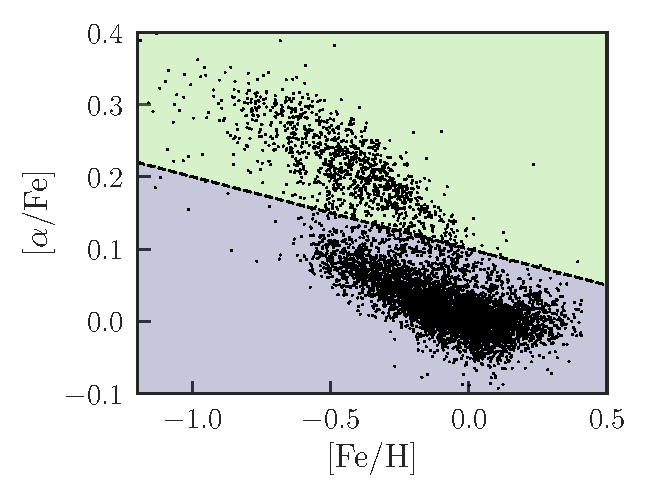
\includegraphics[width=0.8\textwidth]{thesis/Plots/afe_split_colors.pdf}
    \caption[The \feh{} and \afe{} abundances of stars in the solar vicinity from APOGEE DR14, indicating the bimodality in \afe{} at fixed \feh{}]{The \feh{}-\afe{} plane for stars located near the Sun (within 1 kpc) from the fourteenth data release (DR14 of the APOGEE survey). The coloured regions indicate a rough selection of stars with high (\emph{green}) and low (\emph{blue}) \afe{}. A bimodality in \afe{} is clearly present, at fixed \feh{}, between $-0.5 \lesssim \mathrm{[Fe/H]} \lesssim 0.0$ dex. The two populations appear to overlap at roughly solar \feh{}.}
    \label{fig:afe_split}
\end{figure}

These populations have, of course, been studied extensively since their discovery \citep[e.g.][]{1998A&A...338..161F,2003A&A...410..527B,2005A&A...433..185B,2013A&A...560A.109H,2014A&A...562A..71B,2014A&A...564A.115A,2014ApJ...796...38N,2015ApJ...808..132H} and, as expressed in Section \ref{sec:disksize}, have important links to the spatial structure of the Galaxy. Along with the MDFs (mentioned above), large scale spectroscopic surveys have also unveiled the stellar \feh{}-\afe{} distribution over great extents of the disk.  \citet{2014ApJ...796...38N} demonstrated that the positions of Red Clump (RC) stars (whose distances can be accurately measured by the fact that they are standard candles) in \feh{}-\afe{} space change as a function of Galactocentric radius and height. \citet{2015ApJ...808..132H} followed up on that work by showing a similar trend in a much larger sample Red Giant Branch stars. The findings of both studies were that that the mean \feh{} of the low \afe{} stars appears to move to higher \feh{} at smaller $R$, while the high \afe{} stars dominate the distribution at high $z$, and occupy a similar locus everywhere in the disk but appear to decline in density with $R$. These results place very strong constraints on any model which hopes to explain the origin of these element abundance trends, and I will briefly discuss such models in Section \ref{sec:galacticarchaeology}.

\subsection{The Bulge and Bar}

I discuss the bulge of the Milky Way in coordination with the bar, as these components are co-spatial in the center of our Galaxy and have a history and origin which is likely linked in some way, at some point in time.

\subsubsection{Classical or \emph{pseudo}-bulge?}
During the early years of studying the Milky Way bulge, there was much debate as to its origin. The main arguments were either that it built up in the early history of the Galaxy through the merging of its satellite galaxy progenitors -- and thus is a `classical' bulge, resembling the structure of elliptical galaxies, which are thought to be built by the same process -- or that it formed in a secular fashion from stars in the disk or bar of the galaxy to become a `pseudobulge' \citep[a useful summary of these definitions is provided in Section 1.1 of][]{2004ARA&A..42..603K}. There now exists a wealth of evidence to suggest that while external galaxies certainly do host classical bulges \citep[e.g.][]{2009MNRAS.393.1531G}, the Milky Way itself is more likely host to a bulge with a structure indicative of secular processes - a pseudobulge. The Galactic bulge is boxy in shape \citep[e.g][]{1995ApJ...445..716D}, and is proposed to be formed via the heating of stars by buckling of a bar which formed from the stellar disk \citep[e.g.][]{1981A&A....96..164C,1991Natur.352..411R}.



\subsubsection{Unveiling the bar}


\subsection{The Halo}

\subsection{The Local Group}

\section{Galactic archaeology: fossilised galaxy formation}
\label{sec:galacticarchaeology}
\subsection{A schematic for the formation of disk galaxies}

A useful way to present the wealth of work on the formation of the Milky Way is to describe a schematic of its formation as a disk galaxy, as unveiled by studies of it throughout the last century. The conception of the `canonical' model for the birth of the Milky Way in a rapid collapse of a proto-galactic gas cloud \citep[the ELS model;][]{1962ApJ...136..748E} makes a good starting point for such a schematic. 

In what can be considered as the first implementation of Galactic archaeology, \citet{1962ApJ...136..748E} showed that the orbital energies and eccentricities of stars with lower metallicities were increased, inferring that these stars were members of the first generation of stars formed from the originally rapidly collapsed protocloud of our galaxy. The later work of \citet{1978ApJ...225..357S}, which inferred that the varying element abundances of Galactic globular cluster (GC) systems, suggested a different view of the formation of the galaxy through the conglomeration of `protogalactic fragments'. These seminal works underpin many of the modern studies of the Milky Way, and are commonly framed as competitive scenarios. However, at the time, these findings mirrored the developments in the CDM model \citep{1978MNRAS.183..341W}, and analytical models of the collapse of gas in a halo which gained angular momentum from hierarchical clustering produced seemingly realistic disks \citep{1980MNRAS.193..189F}. While analytic approaches would work well at describing galaxy disk formation, hydrodynamical simulations in a cosmological context struggled to produce realistic populations of disk galaxies until advances in the inclusion of detailed feedback models, as expressed in Section \ref{sec:galaxyhaloconnect}. 




%\chapter{The age-resolved spatial structure of the Milky Way disc}
\label{chapter:apogeestruc}
\section{Introduction}

As has already been discussed in Chapter \ref{chapter:intro}, understanding of the present day spatial, kinematic and chemical configuration of the stars of the Milky Way disc is a cornerstone of Galactic archaeology, placing key constraints on models of galaxy disc formation and evolution. Much of our understanding of the time evolution of galaxy discs like that of the Milky Way has arisen from studies which match galaxies of a given stellar mass at $z=0$ to their progenitors at higher $z$ \citep[and therefore, lookback time, e.g.][]{2013ApJ...771L..35V,2015ApJ...803...26P,2016MNRAS.462.4495H}. 
%However, the Sun's position in the Milky Way presents a high-fidelity insight into the structure of a Galactic disc on a star by star basis, which has provided a great many insights into the problem \citep[e.g.][]{1962ApJ...136..748E,1993A&A...275..101E,2013A&A...560A.109H}. 
Data for large numbers of disc stars over a wide range of Galactocentric distances, including positions, chemical abundances and stellar ages are now readily available, due to the advent of modern spectroscopic surveys such as APOGEE \citep{2015arXiv150905420M}, Gaia-ESO \citep{2012Msngr.147...25G} and GALAH \citep{2016arXiv160902822M}, with many future instruments planned, such as WEAVE \citep{2014SPIE.9147E..0LD} and MOONS \citep{2012SPIE.8446E..0SC}, aiming to bolster the revolutionary data releases from \emph{Gaia} \citep{2016A&A...595A...1G}.

In Section \ref{sec:discsize}, I touched upon the definition of the disc population being measured in the Galaxy appears to have a great effect on estimates of it's structure. Thicker stellar populations, defined geometrically have generally flatter radial profiles with larger scale lengths \citep[e.g.][]{2008ApJ...673..864J} than, for example, the populations enhanced in $\alpha$-element abundances \citep[e.g.][]{2012ApJ...752...51C,2012ApJ...753..148B,2016ApJ...823...30B}. Theoretical results have suggested that such \emph{geometric} thick discs are formed from embedded flaring of co-eval populations  \citep{2015ApJ...804L...9M}. The finding of a radial age gradient above the midplane in the disc \citep[e.g.][]{2016arXiv160901168M}, provides further evidence that the \emph{geometric} thick disc is likely to really be a combination of young and flared, and old, centrally concentrated and thick, populations \citep[as predicted by the models of][]{2015ApJ...804L...9M}.

% When considered \emph{in toto}, nearby galaxy discs, and the Milky Way disc, are observed to have a two-component vertical spatial structure, commonly referred to as the \emph{geometric} `thick' and `thin' discs \citep{1979ApJ...234..842T,1979ApJ...234..829B,1982PASJ...34..365Y,1983MNRAS.202.1025G,2008ApJ...673..864J}. Classically, the `thick' components have been characterised by older, kinematically hotter stellar populations, enriched in \afe{}, whereas the `thin' populations assume lower, near solar \afe{} and are kinematically cooler \citep[e.g.][]{2005A&A...433..185B}. It has, however, also been posited that these populations are in fact composed of multiple sub-populations that smoothly span this range of properties \citep[e.g.][]{1987ApJ...314L..39N,1991PASP..103...95N,2012ApJ...755..115B,2012ApJ...753..148B,2016ApJ...823...30B}, thus, in terms of structural parameters, the disc cannot be characterised as the superposition of two distinct structures with different scale heights \citep{2012ApJ...751..131B}. It has been shown  that the total vertical stellar spatial distribution resulting from the overlap of such sub-populations is consistent with a double exponential \citep[see, e.g., Figure 14 of][]{2013A&ARv..21...61R}. It is difficult to explain the presence of a continuity in structure alongside the discontinuity in chemistry seen in the Milky Way.

The Milky Way disc has a complex chemical structure which connects to its spatial structure in a seemingly complex way, with a bimodality in \afe{} seen at fixed \feh{} across many of the observable regions of the disc, that changes in nature with Galactocentric radius and height above the midplane \citep{2003A&A...410..527B,2005A&A...433..185B,2014ApJ...796...38N,2015ApJ...808..132H}. This characteristic feature, and its spatial variation, is difficult to explain using one-zone Galactic chemical evolution (GCE) models \citep[most recently shown by][]{2016arXiv160408613A}, giving rise to attempts to explain it by means other than pure chemical evolution. Examples of such models include the heating of an old, high-\afe{} disc by high redshift mergers \citep[e.g.][]{2004ApJ...612..894B,2008MNRAS.391.1806V,2009ApJ...700.1896K,2013A&A...558A...9M} and the formation of a dual disc by gradual accretion of stars into disc orbits \citep[e.g.][]{2003ApJ...597...21A}. More recent work has also framed this bimodality as a consequence of discontinuous radial migration of stars in the disc \citep{2016arXiv161009869T}. While this chapter examines the structure of the high and low-\afe{} components, I will return to this feature in Chapter \ref{chapter:eagle}.

% However, such chemical structure can be replicated in part by invoking various Galactic chemical evolution models that do not rely on a `one-zone' approximation \citep[e.g.][]{1997ApJ...477..765C,2000A&A...355..929P,2016arXiv160408613A,2016arXiv160407435W}. For example, \citet{2016arXiv160408613A} showed that a combination of GCE models with varying outflow mass loading parameters and inflow timescales (intended to represent enrichment histories at varying Galactocentric radii) could make a roughly bimodal \afe{} distribution. The same models were shown to present a good explanation of the APOGEE \afe{}-\feh{} plane by \citet{2014ApJ...796...38N}. A deeper understanding of the connection between spatial structure in \afe{} and stellar age selected populations in the Milky Way is necessary to link these results. 

 In this chapter, I present the first dissection of radially extended samples of Milky Way disc stars in age, \feh{} and \afe{}. A strong correlation is observed between stellar age and \afe{} in the solar vicinity \citep{2013A&A...560A.109H}. On the other hand, but also in the solar vicinity, a very large scatter is found around the correlation between age and [Fe/H] \citep[e.g.][]{1993A&A...275..101E,2004A&A...418..989N}. This scatter may be explained by the occurrence of radial migration of stars formed in different disc regions. Thickening of the Galactic disc has been invoked as a consequence of outward stellar radial migration \citep[e.g.][]{2009MNRAS.399.1145S}. However, \citet{2012A&A...548A.127M} argue that the effect is small and that such migration in fact only makes discs flare by a small amount. Similarly, \citet{2016ApJ...823...30B} measured the flaring profile of low-\afe{} stars to only slowly exponentially increase with Galactocentric radius, and suggest that radial migration is likely not a viable mechanism for forming thickened disc components. Flaring has also been shown to arise as a result of satellite infall, which can be a stronger flaring agent than migrations \citep[e.g.][]{2009ApJ...707L...1B}. The understanding of flaring and its connection to the evolution of the Galactic disc is essential, but as yet incomplete. In this chapter, I present new constraints on models of radial migration in the disc by studying its effects on the Milky Way's mono-age stellar populations. 

 Many theoretical studies have attempted to understand the observed structure of mono-abundance populations (MAPs) through the use of hydrodynamics and N-body simulations. Few reproduce the observed bimodality in \afe{} at fixed \feh{}, and so an understanding of this has so far proved difficult. However, certain characteristics of the Milky Way \afe{} distribution are beginning to emerge in the most recent cosmological simulations  \citep{2016arXiv160804133M}. Structurally, the mono-age populations of simulated galaxies show good agreement with the Milky Way \citep[e.g.][]{2013MNRAS.436..625S,2013ApJ...773...43B,2014MNRAS.442.2474M,2014MNRAS.443.2452M}. More recent work has brought into question the applicability of MAPs as a proxy for mono-age populations \citep{2017ApJ...834...27M}, showing that, particularly at low-\afe{}, MAPs may have significant age spreads due to the differential nature of star formation in the disc. I show in this chapter that the structures of mono-age and mono-\feh{} populations in the low and high-\afe{} Milky Way disc components present insights which are complementary to those of the MAPs, into the temporal and chemical evolution processes in the disc.

 Previous work studied MAPs in the Milky Way by analysing samples of SEGUE G-dwarfs \citep{2012ApJ...755..115B,2012ApJ...753..148B,2012ApJ...751..131B} and APOGEE red-clump (RC) giants \citep{2016ApJ...823...30B}. In this chapter, I map the spatial distribution of mono-age, mono-\feh{} populations at low and high-\afe{} using a catalogue containing \feh{} and \afe{} from the twelfth data release (DR12) of the APOGEE survey \citep{2015arXiv150905420M} and ages from \citet{2016MNRAS.456.3655M} for 31,244 red giant stars. I complement earlier work by adapting the method developed by \citet{2016ApJ...823...30B} for RC stars, to enable its application to the full red giant branch (RGB) sample from APOGEE. Stars in the RGB are better tracers of the underlying stellar population than their RC counterparts because of reduced uncertainties in the stellar evolution models. Additionally, because they are generally brighter, they are also observed at greater distances. On the other hand, this means that the method developed by \citet{2016ApJ...823...30B} must be adapted to account for the spread in absolute magnitude over the RGB (whereas RC stars can be considered as a near-standard candle). On the basis of these measurements, I will establish the local mass-weighted age-\feh{} distribution, showing the contributions from both low and high-\afe{} stellar populations.

 In Section \ref{sec:dataa}, I present the APOGEE DR12 data and the distance and age catalogues used for this work. Section \ref{sec:methoda} describes the stellar density fitting method, drawing greatly on work by \citet{2016ApJ...818..130B,2016ApJ...823...30B}. Specifically, I describe the generalities of the maximum likelihood fitting procedure and the calculation of the effective survey selection function for RGB stars in Section \ref{sec:densfit}, the adopted parametric stellar density model in Section \ref{sec:densitymodel}, and the method for calculating stellar surface-mass densities in Section \ref{sec:surfmasscalc}. I present the fitted models in Section \ref{sec:resultsa}, calculating the surface-mass density contributions for each mono-age, mono-\feh{} population. In Section \ref{sec:discussiona} I compare these findings to those in the literature and discuss possible scenarios for the formation of the Milky Way's disc in light of these novel results. Section \ref{sec:conclusionsa} summarises the results and conclusions from this chapter. 


 \section{Data}

\label{sec:dataa}
 \subsection{The APOGEE Catalogue}
 \label{sec:APOGEE}
For this chapter, I use data from the twelfth data release \citep[DR12,][]{2015ApJS..219...12A} of the SDSS-III APOGEE survey \citep[][]{2015arXiv150905420M}, a high signal-to-noise ratio (SNR$>100\ \mathrm{pixel}^{-1}$), high resolution ($R \sim 22,500$), spectroscopic survey of over 150,000 Milky Way stars in the near-infrared $H$ Band ($1.5 - 1.7 \mathrm{\mu m}$). Stars were observed during bright time with the APOGEE spectrograph \citep{2010SPIE.7735E..1CW} on the 2.5m Sloan Foundation Telescope \citep{2006AJ....131.2332G} at Apache Point Observatory. Targets were selected in general from the 2MASS point-source catalog, employing a dereddened $(J-K_S)_0 \geq 0.5$ colour cut (in the fields which are of interest here) in up to three apparent $H$ magnitude bins \citep[for a full description of the APOGEE target selection, see][]{2013AJ....146...81Z}. Reddening corrections were determined for the colour cut via the Rayleigh-Jeans Colour Excess method \citep[RJCE,][]{2011ApJ...739...25M}. Corrections are found by applying the method to 2MASS \citep{2006AJ....131.1163S} and mid-IR data from \emph{Spitzer}-IRAC GLIMPSE-I, -II, and -3D \citep{2009PASP..121..213C} when available and from WISE \citep{2010AJ....140.1868W} otherwise. For this work, distance moduli (which make use of the aforementioned reddening corrections) are taken from the \citet{2015ApJ...808..132H} distance catalogue for DR12 (see Section \ref{sec:distances}). 

 All APOGEE data products employed in this paper are those output by the standard data reduction and analysis pipeline used for DR12. The data were processed \citep{2015AJ....150..173N}, then fed into the APOGEE Stellar Parameters and Chemical Abundances Pipeline \citep[ASPCAP,][]{2016AJ....151..144G}, which makes use of a specifically computed spectral library \citep{2015AJ....149..181Z}, calculated using a customised $H$-band line-list \citep{2015ApJS..221...24S}. Outputs from ASPCAP are analysed, calibrated and tabulated \citep{2015AJ....150..148H}. The output \afe{} and \feh{} abundances for DR12 have been shown to have a high degree of precision (at least between $4500 \lesssim \mathrm{T_{\mathrm{eff}}} \lesssim 5200$ K), such that $\sigma_{\mathrm{[Fe/H]}} = 0.05\ \mathrm{dex}$ and $\sigma_{\mathrm{[\alpha/Fe]}} = 0.02\ \mathrm{dex}$ \citep{2016ApJ...823...30B}. I apply here the same external calibrations to \afe{} and \feh{} as \citet{2016ApJ...823...30B}: constant offsets of -0.05 dex and -0.1 dex, respectively. The calibrated, tabulated \feh{} value is used rather than the globally fit $\mathrm{[M/H]}$, which is included in the table.

I then select stars from the DR12 catalogue which were targeted as part of the main disc survey (i.e were subject to the $(J-K_S)_0 \geq 0.5$ cut), have reliably measured abundances (i.e. no warning or error bits set in the ASPCAPFLAG field) and have a well defined distance modulus and age measurement (see Sections \ref{sec:distances} and \ref{sec:ages}, for specific discussion of the age and distance catalogues employed). I apply a secondary cut at $1.8 < \log{g} < 3.0$ to restrict the sample to stars on the red giant branch (RGB), removing most contaminating dwarfs, and very evolved stars near the tip of the RGB. The high end of our $\log{g}$ cut is more conservative than other studies in this regime, however I find this gives the best agreement between the data and stellar evolution models, without significantly reducing the sample size or introducing unwanted bias. These cuts give a final sample of 31,244 stars, spanning $4200 \lesssim \mathrm{T_{\mathrm{eff}}} \lesssim  5050\ \mathrm{K}$ for which the effective survey selection function can be reconstructed.

I further divide the sample into low and high-\afe{} sub-samples, as it has been shown in previous work that the two populations have quite different structural parameters \citep{2016ApJ...823...30B}, and as such it makes sense to proceed to fit their mono-age, mono-\feh{} sub-populations separately. I visually separate the low and high-\afe{} populations, leaving a gap between the two samples of 0.05 dex in \afe{} at each \feh{} (this separation is shown in Figure \ref{fig:afe_feh}), minimising contamination between the subsamples, particularly at the high \feh{} end, where the two populations partially overlap, and at the low \feh{} end, where \afe{} errors become enlarged. The final density fits are performed on finer bins in age and \feh{}, which is defined in Section \ref{sec:ages}. As the adopted separation in \afe{} removes 6532 stars from the full count, when calculating the surface-mass density contributions from the stellar number counts in each age-\feh{} bin, I remove the separation in \afe{}, using the star counts as if the populations were separated along the midpoint of the division (as shown by the dot-dashed line in Figure \ref{fig:afe_feh}). 

 \begin{figure}
  \centering
 	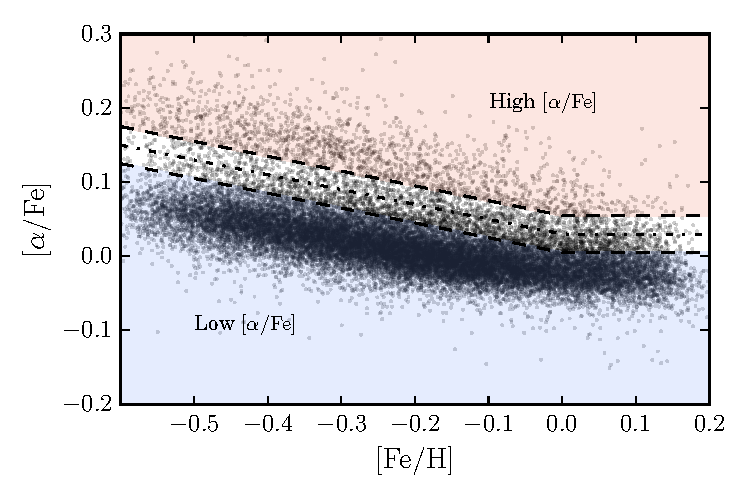
\includegraphics[width=0.7\columnwidth]{afe_feh_subsamples.pdf}
    \caption[\afe{}--\feh{} for the APOGEE DR12 sample, demonstrating the division used to divide between high and low-\afe{} populations in Chapter \ref{chapter:apogeestruc}]{The full APOGEE DR12 RGB sample in \afe{}--\feh{} space. The coloured regions show the division between low and high-\afe{} subsamples used for the DR12 dataset, which is determined by eye to best divide the two populations at the low \feh{} end. At each \feh{} the division between the samples is \afe{} $= 0.05 \ \rm{dex}$, roughly twice the mean uncertainty on \afe{} abundance determinations in APOGEE DR12. The bimodality in \afe{} at fixed \feh{} is visible across many \feh{}, and the lower number of stars in the high-\afe{} sample is clear from this plot. Figure \ref{fig:afe_split} shows a similar sample using the DR14 data, which will be used in Chapter \ref{chapter:highe}.}
 \label{fig:afe_feh}
\end{figure}


The method used to model the spatial density of the mono-age, mono-\feh{} populations, discussed in Section \ref{sec:methoda}, corrects for selection effects induced by interstellar extinction (in addition to the RJCE reddening corrections) using 3D dust maps for the Milky Way derived by \citet{2006A&A...453..635M} for the inner disc plane, combined with those for a large majority of the APOGEE footprint by \citep{2015ApJ...810...25G}, adopting conversions $A_H/A_{K_S}=1.48$ and $A_H/E(B-V) = 0.46$ \citep{2011ApJ...737..103S,2013MNRAS.430.2188Y}.  Fields with no dust data (of which there are $\sim 10$) are removed from the analysis. \citet{2016ApJ...823...30B} discuss the relative merits and limitations of these dust maps as opposed to others which are available, and determine that this combination of dust maps provides the best density fits.


 \subsection{Distance estimates}
 \label{sec:distances}
 
  \begin{figure}
 \centering
 	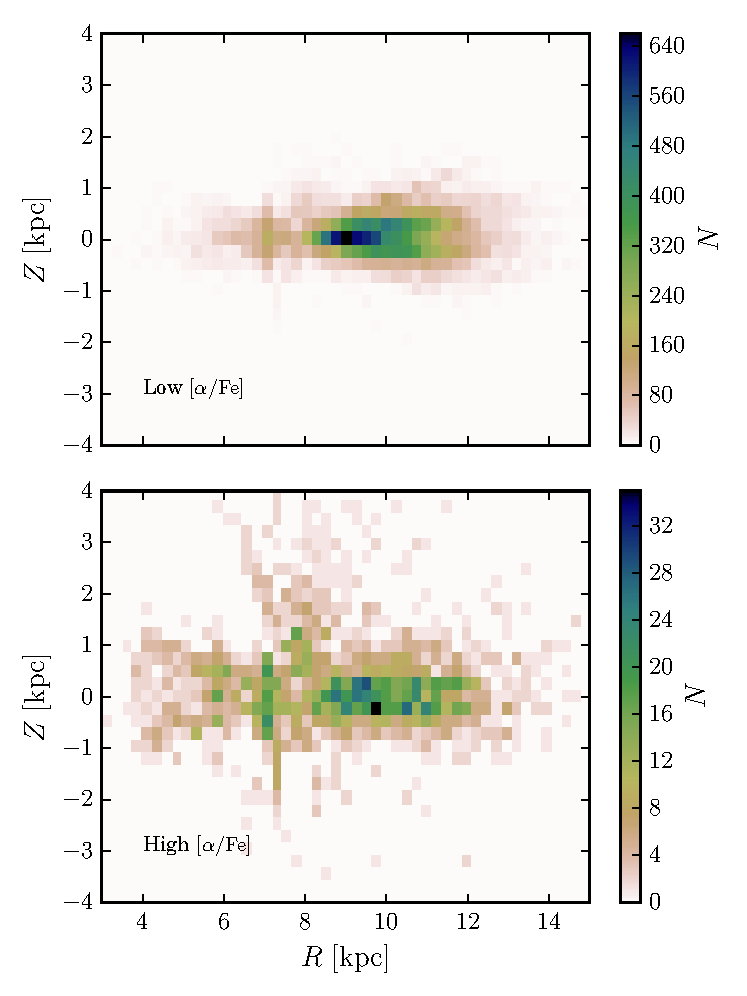
\includegraphics[width=0.8\columnwidth]{spatial_clean_subsamples_binned.pdf}
     \caption[The Galactocentric $R$ and $z$ distribution of stars in the APOGEE DR12 high and low-\afe{} populations]{2D histograms of the spatial distribution (in Galactocentric $R$ and $Z$) of the high and low-\afe{} subsamples from APOGEE DR12, shown in Figure \ref{fig:afe_feh}. The high-\afe{} sample appears more diffuse and extended in height even before selection effects are accounted for. Readers should notice the different colour scale adopted for each panel, due to the much lower number of stars in the high-\afe{} sample.}
     \label{fig:spatial}
 \end{figure}
In this chapter, I use distance estimates from \citet{2014AJ....147..116H} \citep[But see also][for further description]{2015ApJ...808..132H}. Distances are estimated by computing the probability distribution function (PDF) of all distance moduli to a given star using a Bayesian method applied to the spectroscopic and photometric parameters from the DR12 catalogue and the PARSEC isochrones \citep{2012MNRAS.427..127B}. The distance estimates are found to have accuracy at the $15-20\%$ level, upon comparison with cluster members of well known distance observed by APOGEE. 

I use the median of the posterior PDF (which is given in the output catalogue) as the estimate for the distance modulus, and compute the Galactocentric cylindrical coordinates, $R, \phi\ \rm{and}$  $Z$ for each star using the $l,b$ coordinates provided in the APOGEE-DR12 catalogue. The spatial distribution of the two \afe{} sub-samples is shown in Figure \ref{fig:spatial}. I perform a simple cross match between our sample and the APOGEE red clump (RC) value added catalogue (VAC) \citep{2014ApJ...790..127B} and plot the red-clump derived distance ($D_{RC}$) against the estimate from \citet{2014AJ....147..116H} ($D_{MH}$) in Figure \ref{fig:distcomp}. The majority of the \citet{2014AJ....147..116H} distances compare well to the RC distances, but there are notable differences. The \citet{2014AJ....147..116H} distances can be underestimated by as much as 50\%, and I find that $\sim20\%$ of the sample have distances which are underestimated by more than 10\%. Our density fitting method is insensitive to uncertainties on the distances at these scales, as the scale of any variations in the density distribution can be assumed to be far greater than the distance uncertainties. 

 Figure \ref{fig:distcomp} also shows that there is a systematic offset between the RC and \citet{2014AJ....147..116H} distances of the order $\sim 5\%$ across the full range of distances. Adopting this offset as a correction to the distances makes little impact on the final results, merely broadening fitted density profiles slightly, spreading the star counts over a wider Galactocentric distance, meaning that the final stellar surface-mass density estimates are unchanged.

\begin{figure}
 	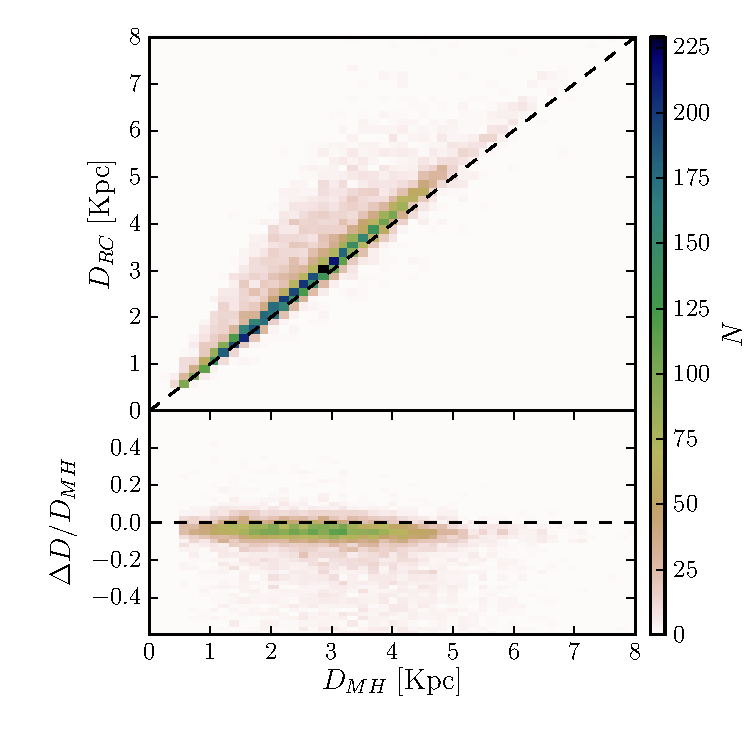
\includegraphics[width=0.8\columnwidth]{distancecomparison_binned.pdf}
    \caption[Comparison of APOGEE RC catalogue distances with distances derived by \citet{2015ApJ...808..132H}, as used in Chapter \ref{chapter:apogeestruc}]{Comparison of APOGEE red clump catalogue (APOGEE-RC) distances $D_{RC}$ with distances derived by \citet{2015ApJ...808..132H}, $D_{MH}$. The top panel directly compares the distances, where the bottom panel shows the difference as a fraction of $D_{MH}$, as a function of that distance.  There are many stars with good agreement, but a distinct fraction of MH distances are underestimated compared to RC ($\sim 20\%$ with distances underestimated by more than $\sim 10\%$). As the variations in the density occur on scales which are, in general, far larger than these discrepancies, these are not problematic in our analysis. The two distance scales differ systematically by a factor of $\sim 5\%$, but this is not corrected for in the following discussion and it does not impact any of the general results.}
    \label{fig:distcomp}
 \end{figure}

Given that stellar distances are rapidly being improved by the \emph{Gaia} mission, it is likely that the precision on stellar distance estimates can now be improved, particularly for stars very close to the sun. However, it is expected that even with parallax information for the stars, the distance estimates to the furthest stars in this sample would likely still be subject to uncertainties of $\sim 5$ to $10\%$ until the highest precision parallaxes become available with the end-of-mission \emph{Gaia} data releases. Given, as I have already pointed out, that the stellar density (which is fitted here) varies on scales far greater than the distance uncertainties, it could be expected that improved precision on distances would only marginally improve the precision and accuracy of the results found here.

 \subsection{Age estimates}
 \label{sec:ages}
I use age estimates for APOGEE DR12 estimated by \citet{2016MNRAS.456.3655M}, who derive an empirical model for the $\mathrm{[C/N]} -M_*$ relation using asteroseismic masses from \emph{Kepler} and abundances from APOGEE for their overlapping samples \citep[APOKASC ][]{2014ApJS..215...19P}. Masses are predicted for DR12 stars which meet quality and stellar parameter criteria outlined in \citet{2016MNRAS.456.3655M}, and ages are estimated from that mass using the PARSEC isochrones with the nearest metallicity to that of the given star. \citet{2016MNRAS.456.3655M} use this empirical relation to build a model which predicts mass and age as a function of $[\text{[M/H], [C/M], [N/M], [(C+N)/M],}\log{g},T_{\mathrm{eff}}]$. It is important to note here that \citet{2016MNRAS.456.3655M} derive a model and fit for the ages in DR12 using the uncalibrated, raw stellar parameters, found in the FPARAM arrays in the APOGEE catalogue. This is difficult to account for when using the age catalogue alongside the calibrated parameters, and must be borne in mind in future comparisons of this work with models and observational results. In addition to this, \citet{2016MNRAS.456.3655M} also mention that care should be taken when applying these ages to regions of the Milky Way where the chemical evolution may have been complex (e.g. the Bulge/Bar region). However, in their Figure 12, they compare the [C/N] ratio as a function of [M/H] in a sample of pre-dredge-up giants in the inner and outer disc, showing that the shapes of the distributions are similar. This suggests that differences in chemical evolution do not affect the $\mathrm{[C/N]}$-age relation within a wide range of galactocentric distances. Therefore, the assumption that it is safe to adopt the \citet{2016MNRAS.456.3655M} ages over the extent of the disc covered by our sample is robust, regardless of the fact that they are trained on the \emph{Kepler} sample, which is limited in its spatial extent.

 Although individual uncertainties on ages are not given in the catalogue, \citet{2016MNRAS.456.3655M} state that the model predicts ages with r.m.s errors of $\sim 40\%$. Although uncertainties are potentially very large at high age, the sample used here is binned with $\Delta \text{age}= 2$ Gyr in order to gauge general trends with age. It should be understood that such trends are smoothed by the age uncertainties, particularly at high age, and detailed comparisons to models should take this age uncertainty into account. I discuss the effect of these uncertainties on our recovered trends with age in Appendix \ref{sec:ageerror}, and show that the methodology still reliably recover such trends with age, even though mixing between bins may be present in the data.

 Figure 11 of \citet{2016MNRAS.456.3655M} shows that there is a significant bias in the ages returned by the model, such that ages are underpredicted at high age when compared to the training set. For this reason, I fit for and apply a correction to the catalogued ages before performing the density fitting procedure. Using Table 1 from \citet{2016MNRAS.456.3655M}, I perform a non-parametric lowess fit to the predicted age--true age distribution. This fit is then used to derive age corrections as a function of predicted age. The fitted correction is shown in Figure \ref{fig:correction} in both predicted vs. true age space and also in $\Delta$ age against the predicted age. The correction as a function of predicted age is then applied to each of the ages in the DR12 catalogue. In all further analysis, I refer only to the corrected ages. The main effect of this correction is to make the high-\afe{} stars older. Consequently, our surface-mass density estimates (presented in Section \ref{sec:surfmassdens}) become more conservative, as the mass contribution per star in older bins is lower (as discussed in Section \ref{sec:discrepant}). \citet{2016MNRAS.456.3655M} comment on the bias in the context that the ages returned for high-\afe{} stars appear younger than previous estimates \citep[from][]{2013A&A...560A.109H,2014A&A...562A..71B,2014A&A...565A..89B}. This correction brings these data more in line with those estimates.  
 
  \begin{figure}
 	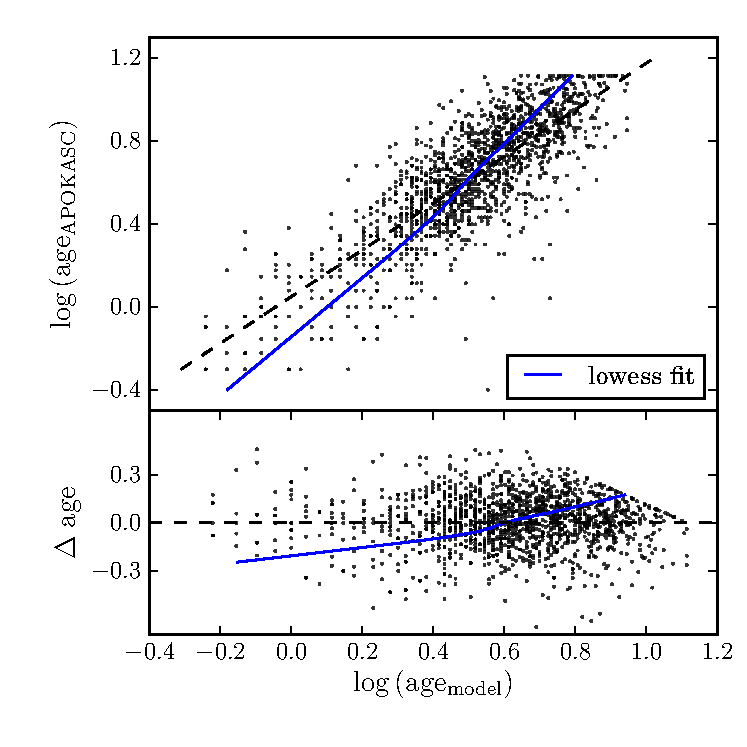
\includegraphics[width=0.8\columnwidth]{agebias_invsout.pdf}
 	\centering
     \caption[Comparison between the input and output ages from \citet{2016MNRAS.456.3655M}, demonstrating the fit and correction which is applied to the age catalogue for APOGEE DR12]{Asteroseismically determined ages from APOKASC against the $\mathrm{[C/M]}$ and $\mathrm{[N/M]}$ based ages from \citet{2016MNRAS.456.3655M}. The line gives the fitted correction for ages from \citet{2016MNRAS.456.3655M}, based on the values for the APOKASC training set, given in their Table 1. The data are fit using a non-parametric lowess fit. Before corrections, older ages are under-predicted, and young ages are over-predicted. The corrections mainly change the scaling of the ages, such that the high-\afe{} sample occupies an age range more in-line with the existing literature \citep[e.g.][]{2016arXiv160407771A,2013A&A...560A.109H} }
  \label{fig:correction}
\end{figure}



 It is also important to account for all other cuts made by \citet{2016MNRAS.456.3655M} on the stellar parameters in the APOGEE catalogue, outlined in full at the beginning of their Section 6.2. While I account for cuts in $T_{\mathrm{eff}}$ and $\log{g}$ by applying the same cuts to the isochrone grid when calculating surface-mass density contributions, it is not possible to properly account for cuts made on the stellar abundances in this way. 9,041 stars are removed from the 40,285 star catalogue (those with distances, after the $\log{g}$ cut mentioned above) by these abundance cuts, to give the final catalogue size of 31,244. This means that $\sim 25\%$ of genuine star counts are missing from the age catalogue, and therefore unaccounted for in the following analysis. With no robust method for determining the age distribution of these missing stars, I make the simplest assumption that these star counts can simply be added uniformly to each age-\feh{} bin. I make this correction by simply increasing the counts in each bin by $25\%$ when calculating the surface-mass density. This correction simply acts to increase the final surface-mass density values systematically by $25\%$.

Another important consideration when using this set of ages regards stars whose chemical compositions are such that the ages fit from the model (after making the corrections) would be higher than 13 Gyr and left out of the analysis. As age estimates are computed based on the surface parameters and abundances of the stars using a fitting function, many stars with strongly outlying abundances and parameters can be assigned ages which are greater than 13 Gyr. I find that the 3020 such stars (in the final sample) have an average [C/Fe] which is lower than the general sample, and an average [N/Fe] which is enhanced with respect to the stars with reliably measured ages. I also find that at fixed \feh{} and $\log{g}$ these stars have warmer $T_{\mathrm{eff}}$. While these properties are expected given their age measurements, there is a distinct possibility of some peculiarity of these stars. For example, if such stars were early AGB stars \citep[having gone through the second dredge-up, reducing the surface C abundance, e.g.][]{1999ApJ...510..232B}, which had been fit as RGB stars, their actual age may be considerably younger, and their counts missed in the younger bins (where mass contribution per star is higher). As the nature of these stars is debatable and a correction cannot be made confidently before carrying out the full analysis, the missing counts from these stars are regarded as a contribution to the systematic error budget, which is discussed fully in Section \ref{sec:discrepant}.

I demonstrate the adopted binning in (age,[Fe/H]) space in Figure \ref{fig:numbins}, showing also the number of stars which fall in each bin and the general distribution of stars in (age,[Fe/H]) space. There is a notable separation in age between the high and low-\afe{} subsamples. 


 \begin{figure}
 	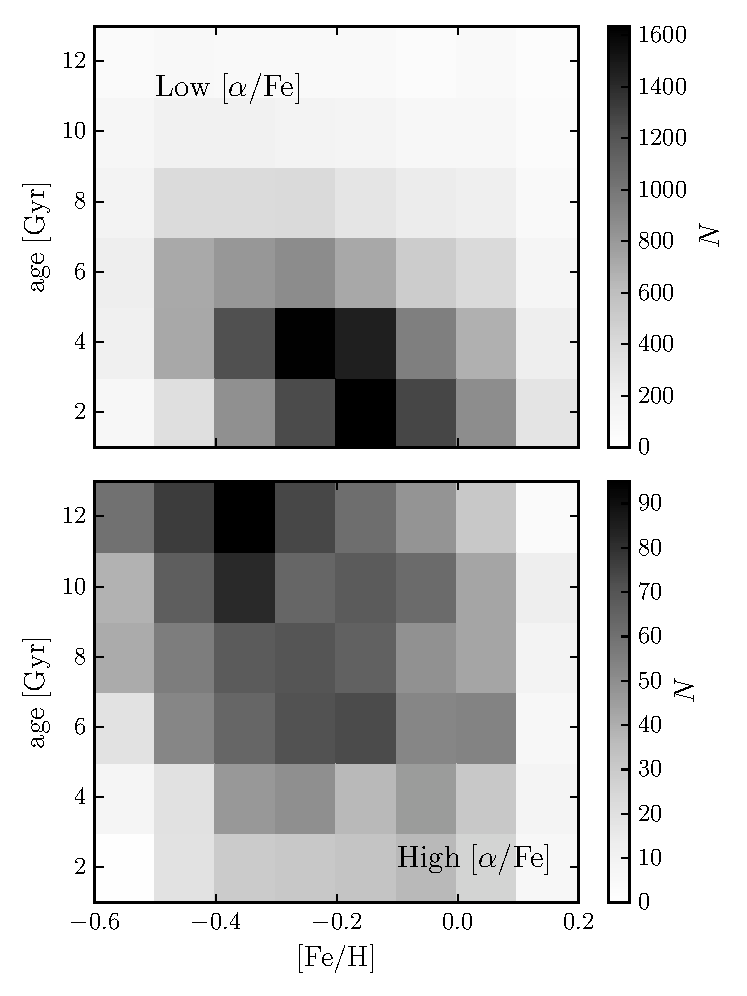
\includegraphics[width=0.8\columnwidth]{agefeh_numbins.pdf}
     \caption[2D Histogram demonstrating the number of stars in each age and \feh{} bin, in the high and low-\afe{} populations, adopted for modelling the stellar density in the disc]{2D Histograms showing the raw number of stars in each (age,\feh{}) bin of the low (\emph{left}) and high (\emph{right}) \afe{} sub-samples. I draw the reader's attention to the difference in amplitude between the two sub-samples (and the associated difference in colour scale normalisation). Although the majority of bins are well sampled ($\gtrsim 30$ stars), there are some greatly undersampled bins, for which well-defined fits are not possible. }
    \label{fig:numbins}
 \end{figure}

 \section{Method}
 \label{sec:methoda}
 In this section I describe the method for fitting the underlying number density of stars in the Milky Way from APOGEE observations, which is represented here as $\nu_*(X,Y,Z|\theta)$, in units of stars kpc$^{-3}$. The calculation of this quantity requires allowances to be made for the survey selection function, which is non-trivial due to the presence of inhomogeneous dust extinction along lines of sight observed by APOGEE, the invocation of different $H$ magnitude limits in the target selection, and the use of RGB stars as a tracer - which cannot be considered as standard candles, as is done for the RC sample. The quantity which I am ultimately interested in is the surface-mass density of stars at the solar radius, $\Sigma_{R_0}$, in units of $\mathrm{M_{\odot}}\ \mathrm{pc^{-2}}$, which I infer here from the number of stars in the APOGEE sample as a function of position. I describe the method for this calculation in Section \ref{sec:surfmasscalc}. The methodology presented here consists of an adaptation of that used by \citet{2016ApJ...823...30B}, employing a modified version of their publicly available code\footnote{Available at \url{https://github.com/jobovy/apogee-maps} - and updated to include the adapted analysis used here}. Although the general method is identical, I describe again the key components for clarity and completeness.

The procedure, described in full below, can be summarised as follows:
  \begin{itemize}
  \item Parametric density models are fit to the APOGEE star counts using a maximum likelihood fitting procedure, based on the assumption that star counts are well modelled as an inhomogeneous Poisson point process. The density models which I assume throughout the remainder of this chapter are described by radially broken exponentials, with scale lengths $h_{R,\mathrm{[in,out]}}$ either side of a break radius $R_{\mathrm{peak}}$ (where $h_{R,\mathrm{in}}$ denotes the scale length of the inner profile and vice versa), and a vertical distribution which is a single exponential with scale height $h_Z$, which is modified as a function of $R$ by an exponential flaring term with scale length $R_{\mathrm{flare}}$. I show that if the density is better fit by a single exponential, it is recovered as so by this procedure.
 \item A best fit density model is obtained for every bin in age and \feh{}, at high and low-\afe{}. This best fit model is then used to initiate an MCMC sampling of the posterior PDF. I then use the median and standard deviation of one dimensional projections of the MCMC chain as our adopted parameter values and uncertainties.
  \item As the fitting procedure does not fit for the normalisation of the density $N_{R_0}$, the number surface density of stars at the solar radius in stars pc$^{-2}$, I calculate this value by comparing the observed number of stars in each bin to that which would be observed in APOGEE for the fitted density model if $N_{R_0} = 1 $ star pc$^{-2}$. The $N_{R_0}$ for each bin is then converted into the surface-mass density in visible stars at the solar radius $\Sigma_{R_0}$ by converting the mass in RGB stars observed to the total mass using stellar evolution models.
 \end{itemize}

 

 \subsection{Density Fitting Procedure}
\label{sec:densfit}
Initially, the number density of stars is fit for each sub-population shown in Figure \ref{fig:numbins}. The following discussion describes the general procedure used for fitting density models with a generic set of parameters $\theta$. The actual stellar number density model adopted is discussed in Section \ref{sec:densitymodel}. \citet{2016ApJ...823...30B,2012ApJ...753..148B,2013A&ARv..21...61R} have shown that the observed rate of stars as a function of position, magnitude, colour and metallicity can be modelled as an inhomogeneous Poisson point process. Stars are distributed in the space defined by $O = [l,b,D,H,\mathrm{[J-K_S]_0}, \mathrm{[Fe/H]}]$ -- position, magnitude, colour and metallicity -- with an expected rate $\lambda(O|\theta)$ (which has units of stars per arbitrary volume unit in O), parameterised by a set of parameters $\theta$ (which are, in this particular case, the parameters describing an adopted density profile). This rate function is written fully as
 \begin{multline}
 \lambda(O|\theta) = \nu_*(X,Y,Z|\theta) \times |J(X,Y,Z;l,b,D)| \\ \times \rho(H, [J-K_S]_0, \mathrm{[Fe/H]}|X,Y,Z) \times S(l,b,H) 
 \label{eq:rate}
 \end{multline}
 where $\nu_*(X,Y,Z|\theta)$ is the quantity being estimated, which is defined as the stellar number density in rectangular coordinates, in units of stars kpc$^{-3}$. $ |J(X,Y,Z;l,b,D)|$ is the Jacobian of the transformation from rectangular $(X,Y,Z)$ to Galactic $(l,b,D)$ coordinates and $ \rho(H, [J-K_S]_0, \mathrm{[Fe/H]}|X,Y,Z) $ denotes the density of stars in magnitude, colour and metallicity space given a spatial position $(X,Y,Z)$, in units of stars per arbitrary volume in magnitude, colour and metallicity space. $S(l,b,H)$ is the survey selection function (the fraction of stars observed in the survey) which includes dust extinction effects, which I will discuss in the following. When expressed in this way, fitting the density model parameters $\theta$ becomes a maximum likelihood problem.

 The likelihood is a sum over all data-points considered in a given age-\feh{} bin, and gives the likelihood of the parameters $\theta$ given the data. For this application, it is written as
 \begin{multline}
 \ln \mathcal{L}(\theta) = \sum_{i} \left[ \ln \nu_{*}(X_i, Y_i, Z_i|\theta)- \ln \int dO \lambda(O|\theta) \right]
 \label{eq:likelihood}
 \end{multline}
 where second term on the right hand side of the equation, $ \int dO \lambda(O|\theta)$, describes the effective volume of the survey. I drop the other factors in the rate in Equation (\ref{eq:rate}) in the argument of the logarithm, because the other factors do not depend on the model parameters $\theta$. The effective volume is independent of the data-point considered, and is an intrinsic property of the survey for a given $\theta$. It provides the normalisation for the rate likelihood, and is non-trivial to evaluate due to the presence of patchy dust extinction along lines of sight in the survey.

 The effective volume is written generally as
  \begin{multline}
 \label{eq:effvol}
 \int dO \lambda(O|\theta) = \sum_{\text{fields}} \Omega_f \int dD D^2 \nu_*([X,Y,Z](D,\text{field})|\theta)\\ \times \mathfrak{S}(\text{field},D)
 \end{multline}
 which is a sum over all APOGEE fields, where $\Omega_f$ is the solid angle of the field considered. The integrand $ \nu_*([X,Y,Z](D,\text{field})|\theta)$ is the density at each point along a line of sight, assumed to be constant over the angular size of the field. $\mathfrak{S}(\text{field},D)$ represents the effective survey selection function, which is given by the integration of the survey selection function over the area of any given field and is written, in this case, as
 \begin{multline}
 \mathfrak{S}(\text{field}, D) = \sum_k S(\text{field},k) \\ \int dM_H \frac{\Omega_k(H_{\text{[min,max]},k}, M_H, A_H[l,b,D], D)}{\Omega_f}.
 \label{eq:effsel}
 \end{multline}
 This is a sum over the apparent magnitude bins, $k$, in the APOGEE target selection, with the integral representing the fractional area of the APOGEE field where stars are observable, given the distance modulus and extinction at a given position. The term describing this area is $\Omega_k$, which is the observable area of the field at a given distance and absolute magnitude, written as
 \begin{multline}
 \Omega_k(H_{\text{[min,max]},k}, M_H, A_H[l,b,D], D) =\\ \Omega(H_{\text{min},k} - [M_H - \mu(D)] < A_H(l,b,D) < H_{\text{max},k} - [M_H - \mu(D)])
 \end{multline}
 where $H_{\text{[min,max]},k}$ denotes the minimum and maximum $H$ for an apparent magnitude bin $k$ in the APOGEE target selection and $\mu(D)$ is the distance modulus at $D$.  $A_H(l,b,D)$ is the $H$ band extinction at a given position, which I obtain from the 3D dust maps described in Section \ref{sec:APOGEE}. This area is integrated (in Equation (\ref{eq:effsel})) over the full absolute $H$-band magnitude, $M_H$, distribution in an (age,\feh{}) bin. I estimate the $M_H$ distribution for each (age,\feh{}) bin using the PARSEC isochrones \citep{2012MNRAS.427..127B} within that bin, weighted with a \citet{2003PASP..115..763C} IMF. The same cuts in $\log{g}$ and $(J-K_S)_0$ colour are applied to the isochrone points as are imposed on the data, and perform a Monte Carlo integration using the resulting $M_H$ distribution to evaluate the integral in Equation (\ref{eq:effsel}). S(\text{field},k) in Equation (\ref{eq:effsel}) denotes the 'raw' APOGEE selection function, which gives the fraction of the stars in the photometric catalogue that were observed spectroscopically \citep[see][for details]{2013AJ....146...81Z}. This number is constant within an apparent magnitude bin and within an APOGEE field, which is why $S$ is cast as a function of field and magnitude bin in Equation (\ref{eq:effsel}). The values of S(\text{field},k) (and $\mathfrak{S}(\text{field}, D)$) are evaluated using the \texttt{apogee} python package \footnote{Available at \url{https://github.com/jobovy/apogee}}.

$\mathfrak{S}(\text{field}, D)$ is then evaluated over a grid of distances for each APOGEE field for simple computation of $\int dO \lambda(O|\theta)$. The likelihood function in Equation (\ref{eq:likelihood}) is then optimised for a given density model and data-set using a downhill-simplex algorithm, to obtain the best fitting set of parameters $\theta$. A Markov Chain Monte Carlo (MCMC) sampling of the posterior PDF is then initiated using this optimal solution. This is implemented with an affine-invariant ensemble MCMC sampler  \citep{goodmanweare2010,2013PASP..125..306F}. All parameter values and associated uncertainties for individiual (age,\feh{}) bins which are reported in the following sections represent the median and standard deviation $\sigma$, respectively, of one dimensional projections of the MCMC chain. 

 \subsection{Adopted stellar number density models}
 \label{sec:densitymodel}
 It was shown in \citet{2016ApJ...823...30B} that density profiles of MAPs are well represented by axisymmetric profiles that can be written as 
\begin{equation}
 \nu_*(R, \phi, Z) = \Sigma(R)\zeta(Z|R) \quad \text{where } \int dZ \zeta(Z|R) = 1.
 \end{equation}
 Furthermore, the exact form of the best fitting profile is that of a radially broken exponential, with a vertical profile that is an exponential with a scale height which varies exponentially with R (a flaring profile), such that
 \begin{equation}
 \ln \Sigma(R) \propto  \begin{cases}
     -h_{R,\text{in}}^{-1}(R-R_0)    & \quad \text{where } R \leq R_{\text{peak}}\\
   -h_{R,\text{out}}^{-1}(R-R_0)  &\quad \text{where } R > R_{\text{peak}}\\
   \end{cases}
 \end{equation}
 and
 \begin{equation}
 \ln \zeta(Z|R) \propto h_Z^{-1} \exp{(R_{\mathrm{flare}}^{-1}[R-R_0])} |Z|-\ln{h_Z(R)}.
 \end{equation}
$R_0$ denotes the solar radius, which I assume here to be 8 kpc. This number only sets the radius at which the profiles are normalised, and so does not have any effect on the fitting procedure. I adopt the same general set of density profiles to describe the mono-age, mono-metallicity populations which are studied here. I bin in \feh{} to account for the observed \feh{} spread at fixed age \citep[e.g.][and our Figure \ref{fig:numbins}]{1993A&A...275..101E}. \citet{2016ApJ...823...30B} also showed that when mock data were fit using the procedure in Section \ref{sec:densfit} and the density profile above, the input parameters were always recovered within acceptable uncertainty ranges. In particular, mock data generated from a single exponential profile was still recovered as such (i.e. with $R_{\mathrm{peak}} = 0$) even when fit assuming a broken exponential profile.

I also note here that this sample is not limited to stars which are members of any specific Galactic component, and as such, may include small numbers of halo stars in the very high-\afe{} and low \feh{} regimes. However, the fitting procedure is agnostic to these contaminants, which would only cause the fits to have larger uncertainty (from the MCMC exploration) about the best fit from the dominant population in a given bin.

\subsection{Stellar surface-mass densities}
 \label{sec:surfmasscalc}
The surface-mass density in visible stars for each of the age and \feh{} populations is computed using the method originally outlined in \citet{2012ApJ...751..131B}. As the fitting procedure does not fit for the normalisation of the density (the surface density is normalised to 1 at $R_0$), I first compute the normalisation $N_{R_0}$, which represents the number density of stars at the solar radius in units of stars pc$^{-2}$ in an (age,\feh{}) bin. $N_{R_0}$ is given by the relation 
\begin{equation}
 N_{R_0} = \frac{N_{*,\text{observed}}}{\int dO \lambda(O|\theta)}
\end{equation}
where $N_{*,\text{observed}}$ is the number of stars observed in the survey for a given (age,\feh{}) and $\int dO \lambda(O|\theta)$ is the usual definition of the effective volume (given by Equation (\ref{eq:effvol})) for a given set of parameters $\theta$, found using the method in Section \ref{sec:densfit}. 

The contribution to stellar surface-mass density is found by first multiplying $N_{R_0}$ by the average mass of a red giant star in the same range of age and \feh{}, given the selection criteria on $\log{g}$ given in Section \ref{sec:APOGEE} (which picks out the RGB) and  $(J-K_S)_0 \geq 0.5$ (given that I only use fields in which this cut was applied).  I then correct this value to represent the total stellar population by dividing by the fractional contribution of the red giants to the total underlying population. These values are found using PARSEC isochrones \citep{2012MNRAS.427..127B}, weighted with a Log-normal \citet{2001ApJ...554.1274C} IMF, as described in the calculation of the effective volume in Section \ref{sec:densfit}. This then leads to a stellar surface-mass density $\Sigma_{R_0}$ as a function of age and \feh{}. The conversion can be expressed as
\begin{equation}
 \Sigma_{R_0}(\mathrm{age,[Fe/H]}) = N_{R_0} \frac{\langle M_{\text{RGB}} \rangle (\mathrm{age,[Fe/H]})}{\omega(\mathrm{age,[Fe/H]})},
\end{equation}
where $\langle M_{\text{RGB}} \rangle (\mathrm{age,[Fe/H]})$ is the mean stellar mass in an (age,\feh{}) bin, and $\omega(\mathrm{age,[Fe/H]})$ is the fraction of stars in the total stellar population in an (age,\feh{}) bin which are within the $\log{g}$ and $(J-K_S)_0$ cuts in APOGEE. The stellar surface-mass density contributions of each bin can then be summed to give the total stellar surface-mass density at the solar radius $\Sigma_{R_0, \text{tot}}$.

The final surface-mass density estimate is strongly dependent on the conversion factors in the above equations, the average RGB star mass, $\langle M_{\mathrm{RGB}} \rangle$, and the fractional contribution from giants, $\omega$. The average giant masses in the range of age and \feh{} used span $0.9 \lesssim \langle M_{\mathrm{RGB}} \rangle \lesssim 2.1 \mathrm{M_{\odot}}$. The most metal poor and oldest populations have the lowest average mass, and the youngest, most metal rich populations have the highest. The fractional contribution from giants in this regime ranges between $0.002 \lesssim \omega \lesssim 0.02 $. The oldest and most metal poor populations have the least giants, whereas the youngest, metal rich populations have the most. These values appear to sit well with recent inventories of the solar neighbourhood, which suggest giants should make up of the order of a few percent of the mass \citep{2015ApJ...814...13M}. I discuss the potential systematics introduced by the use of stellar evolution models in Section \ref{sec:discrepant}.


\section{Results}
\label{sec:resultsa}
I now present results from the density fitting procedure, and the subsequent calculation of the surface-mass density contribution of each mono-age, mono-\feh{} population in Figure \ref{fig:numbins}. Density fitting is performed on all populations, but I only display here the fits for populations with $> 30$ stars, as data below this level become too noisy to render reliable fits. Although the remaining fits can be noisy when star counts are near this limit, this is reflected in the error analysis arising from the MCMC exploration of the posterior PDF of the fitted parameters. I refer the reader to Appendix \ref{sec:densityfits} for a comparison between the data and the fitted models for each mono-age, mono-\feh{} bin, and a qualitative discussion regarding the rationale behind the decision to discuss fits to only the broken exponential density profile described in Section \ref{sec:densitymodel}.

\subsection{The radial profile of mono-age, mono-\feh{} populations}
The fits to the surface density in the low and high-\afe{} sub-samples are shown in Figure \ref{fig:surfdens}. I display fits for all age and \feh{} bins with $> 30$ stars. By shading the profiles by their surface-mass density contribution (as shown in Section \ref{sec:surfmassdens}), I intend to draw the eye to the profiles which contribute most to the mass of the Milky Way disc. I defer a discussion of the individual mass contributions of each bin to Section \ref{sec:surfmassdens}, concentrating in this section on trends in the shapes of the density profiles. 


Although fit with the broken exponential, high-\afe{} profiles are generally better described by near-single exponentials, either showing no break in the radial range, or being fit by a profile with a break at low significance (i.e. a single line could be drawn through the coloured band). Many of the outer profiles (after $R_{\mathrm{peak}}$) in the high-\afe{} sub-sample appear to have a similar slope, suggesting that they may all be represented by the same exponential. The mean outer scale length for the high-\afe{} populations is $h_{R,\text{out}} = 1.9\pm 0.1$ kpc. The picture is noticeably different in the low-\afe{} sub-sample, with profiles showing clear breaks, at well defined radii. Any trends in break radius in this regime are determined with high significance. low-\afe{} profiles have a density which increases with radius out to the break radius, and declines outward of this radius. The fits are not constrained to behave in this way, and this indicates that mono-age, mono-\feh{} populations at low \feh{} are shaped approximately as donut-like annuli. The variation of the break radius then represents the moving peak of stellar density as a function of age and \feh{}. Concentrating on the bins youngest bin ($1 < \mathrm{age} < 3$ Gyr), the break radius is a declining function of metallicity, moving between $R_{\mathrm{peak}}=10$ kpc at $-0.6 < \mathrm{[Fe/H]} < -0.5\ \mathrm{dex}$ down to $R_{\mathrm{peak}} < 8$ kpc at $0.1 < \mathrm{[Fe/H]} < 0.2\ \mathrm{dex}$. This trend is also present in older bins but with decreased amplitude. In a fixed \feh{} bin, $R_{\mathrm{peak}}$ appears to remain roughly constant (within $\sim1$ kpc) at ages between 1 and 6 Gyr.  At ages older than this $R_{\mathrm{peak}}$ varies in unexpected ways, but there is much less mass contribution from these populations, and I attribute much of this behaviour to noise due to the narrow age bins. 


On the other hand, the low-\afe{} profiles change \emph{shape} (either side of $R_{\mathrm{peak}}$) with age, in a fixed \feh{} bin. The youngest populations show a sharp peak, with a steep increase and decline either side of $R_{\mathrm{peak}}$. As populations grow older, the profile broadens significantly, becoming almost flat in the lowest \feh{} bins. I show this behaviour by finding the inverse of the difference between the inverse outer and inner scale length\footnote{Taking a ratio of the sum of the density at fixed $\Delta R$ either side of $R_{\mathrm{peak}}$ to that at $R_{\mathrm{peak}}$ would give some measure of width. Then, assuming $\Delta R << h_{R,[\text{in,out}]}$, a Taylor expansion of this ratio $\sim \Delta R (h_{R,\text{out}}^{-1}-h_{R,\text{in}}^{-1})$. I then plot the inverse of this factor such that it increases for broader profiles.}, such that a low value denotes a sharper peak, whereas a broader profile has a higher value. I show how this value changes with age for the low-\afe{} populations in Figure \ref{fig:agevsbroadening}. The peak is sharpest in the younger populations, and becomes broader with age. Old populations have artificially sharpened peaks in this diagnostic due to their being better described by single exponentials. Notably also, in Figure \ref{fig:surfdens}, at low \feh{} the inner profiles flatten faster than the outer profile, whereas the higher \feh{} populations show the opposite behaviour. For example, in the $-0.3 < \mathrm{[Fe/H]} < -0.2\ \mathrm{dex}$ bin, the outer profile appears to remain roughly constant in slope between 1 and 6 Gyr, while the inner profile flattens significantly. The opposite is seen in the $0.1 < \mathrm{[Fe/H]} < 0.2\ \mathrm{dex}$ bin, where the outer profile flattens considerably with age. 


\begin{landscape}
\begin{figure}
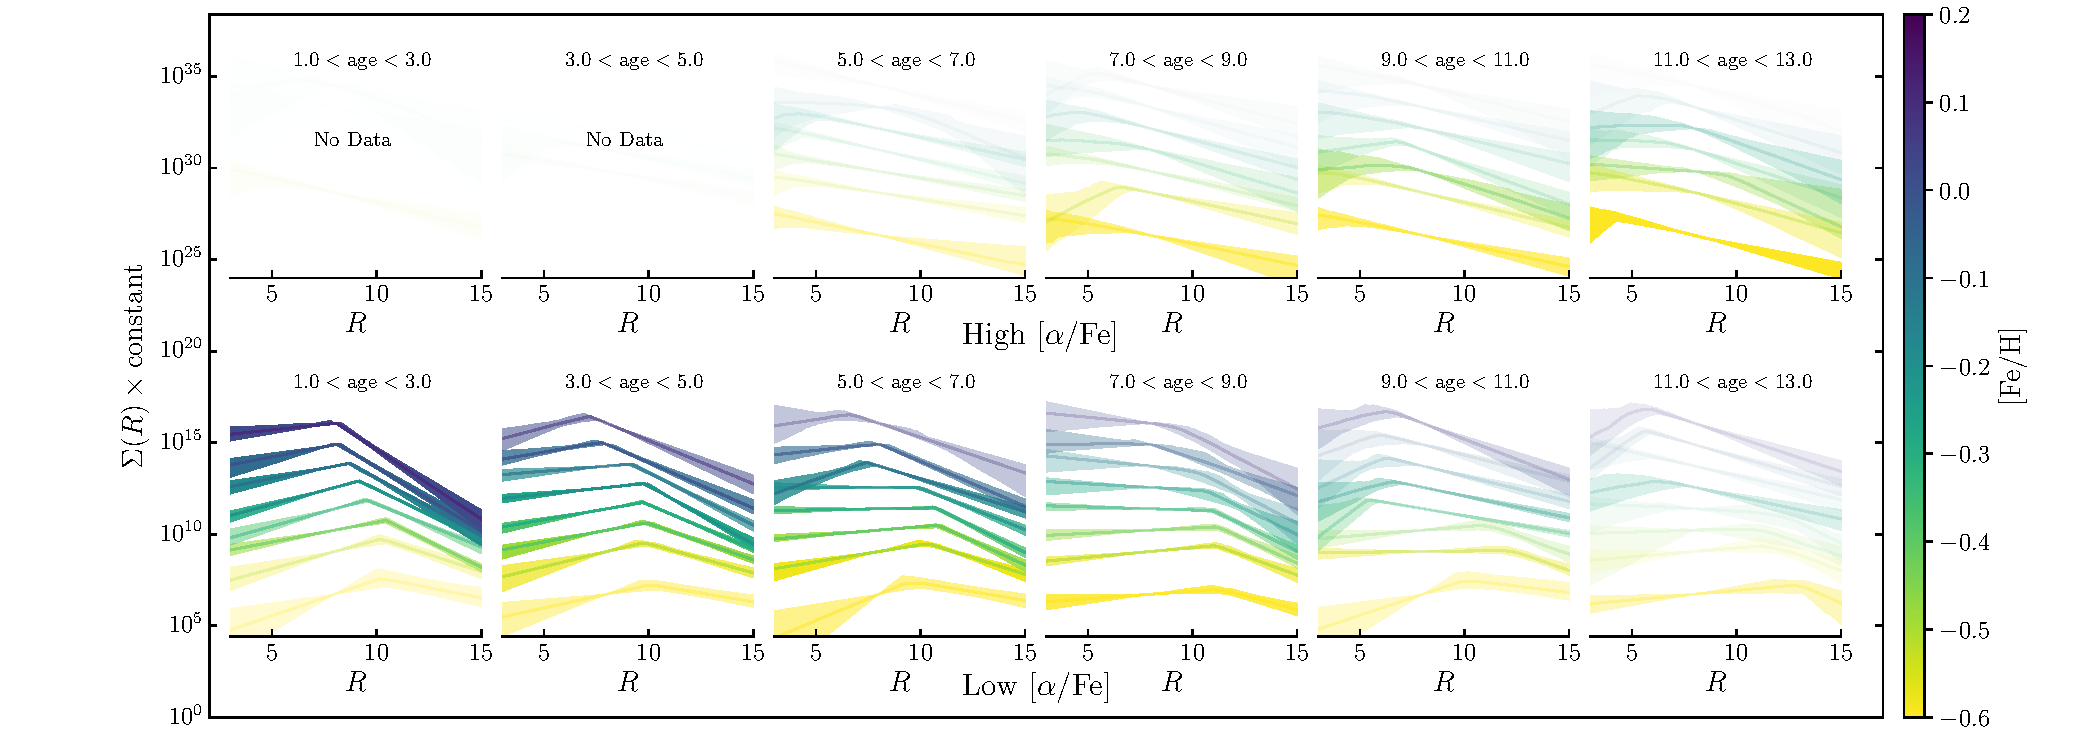
\includegraphics[width=1.0\textwidth]{surfdens_profile_adjusted.pdf}
      \centering
     \caption[Surface density profiles of mono-age, mono-\feh{} populations in the low and high-\afe{} disc components of the Milky Way]{The fitted surface density profiles for the high-\afe{} (\emph{top}) and low-\afe{} (\emph{bottom}) sub-samples as a function of \feh{} (colour) and age (increasing from left to right). The coloured bands represent the 95\% uncertainty range.  Only profiles for bins containing$ > 30$ stars are shown. The profiles have a transparency according to the surface-mass density calculated for each bin in Section \ref{sec:surfmassdens}, normalised separately for each row (i.e. in each \feh{} bin), to draw the eye to those profiles which contribute most to the Milky Way surface-mass density. High-\afe{} profiles are described well by a single exponential, whereas young, low-\afe{} profiles are broken exponentials with a peak density which varies in radius in the disc.}
     \label{fig:surfdens}
 \end{figure}
\end{landscape}


 \begin{figure}
 	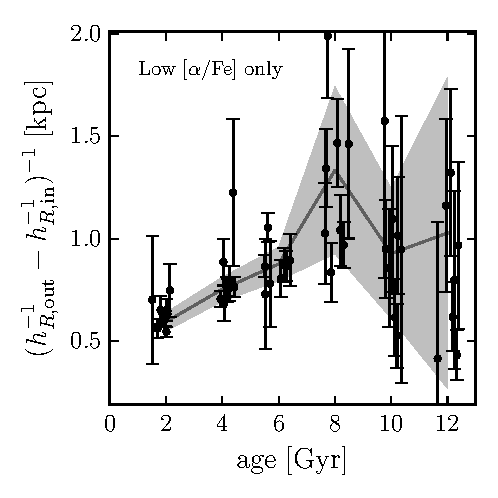
\includegraphics[width=0.6\columnwidth]{broadvsage.pdf}
     \caption[The broadening of surface density profiles as a function of age in the low-\afe{} mono-age, mono-\feh{} populations]{The profile width $(h_{R,\mathrm{out}}^{-1} - h_{R,\mathrm{in}}^{-1})^{-1}$ against age for the low-\afe{} populations (this diagnostic is irrelevant for the high-\afe{} populations, which are generally fit by single exponentials). A small random jitter is added to the central age of each age bin, to make individual points and their uncertainty clearer. The relations and coloured band shows the running surface-mass density weighted mean and standard deviation in the age bins. The profile width increases with age. A higher value of this diagnostic suggests a broader surface density profile, showing that older populations are flatter and broader around the peak density.}
     \label{fig:agevsbroadening}
 \end{figure}



\subsection{The vertical profile of the disc}
I now examine the variation of $h_Z$ as a function of radius in mono-age, mono-\feh{} populations. Because mono-age, mono-\feh{} populations are well described by a single scale height, which is modified by a flaring term $R_{\text{flare}}$, this means that $h_Z$ is weakly dependent on $R$ for profiles which flare. $h_Z$ as a function of $R$ for age-\feh{} bins with $> 30$ stars is shown in Figure \ref{fig:hzprofile}, adopting the same shading as Figure \ref{fig:surfdens} to draw the eye to the profiles with greater mass contribution. The dashed line represents $0.3$ kpc, for reference.

Figure \ref{fig:hzprofile} suggests that the disc is thicker as traced by older populations. All \feh{} bins thicken as age increases. This is clear in the left panel of Figure \ref{fig:agevshzrf}, which shows the surface-mass density weighted mean variation of $h_Z$ with age. The mean $h_Z$ spans the range between 0.2 and 0.8 kpc. The high-\afe{} populations have  a bump in the mean $h_Z$ at 8 Gyr, but $h_Z$ generally increases with age, similarly to the low-\afe{} populations. The shapes of the profiles of the youngest populations in Figure \ref{fig:hzprofile} in the low-\afe{} subsample show little variation with \feh{}, and this trend generally continues to older ages. This is also reflected in the low uncertainties associated with the blue points in the left panel of Figure \ref{fig:agevshzrf}. 


\begin{landscape}
 \begin{figure}
 	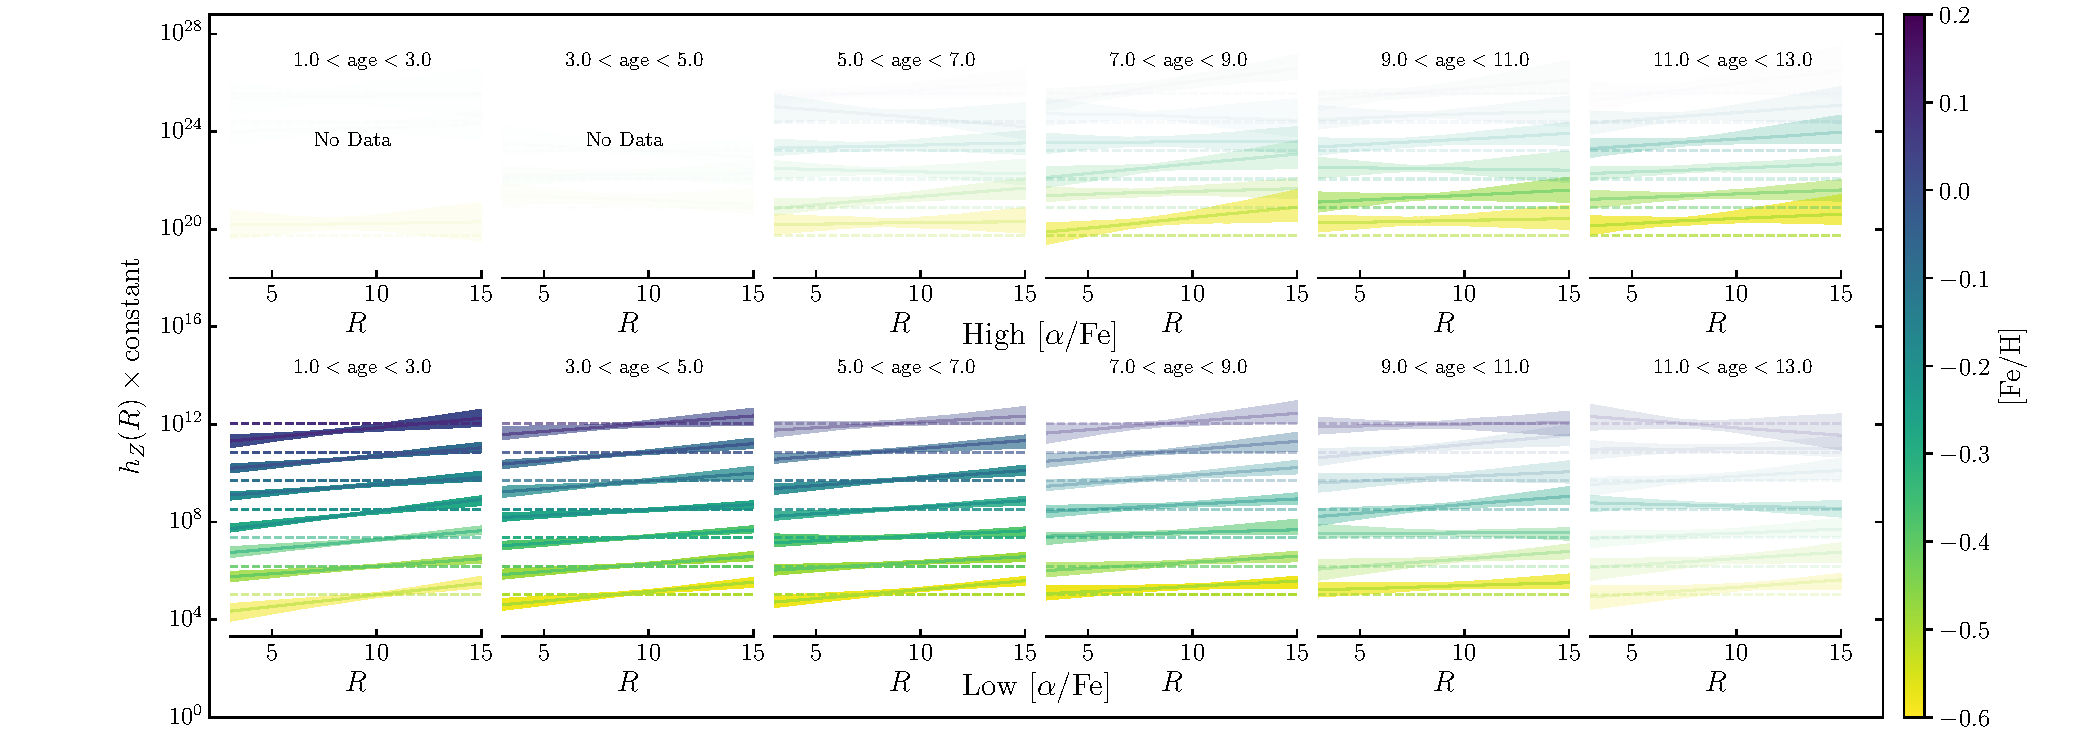
\includegraphics[width=1.\textwidth]{hz_profile_adjusted.pdf}
 	\centering
     \caption[Radial scale height profiles of mono-age, mono-\feh{} populations in the low and high-\afe{} disc components]{Vertical profiles for the high-\afe{} (\emph{top}) and low-\afe{} (\emph{bottom}) sub-samples as a function of \feh{} (colour) and age (increasing from left to right). The coloured bands represent the 95\% uncertainty range. Only profiles for bins with $> 30$ stars are shown, with profiles shaded according to their surface-mass density contributions (discussed in Section \ref{sec:surfmassdens}).  The dashed lines represent $h_Z = 0.3$ kpc, for reference.}
     \label{fig:hzprofile}
 \end{figure}
\end{landscape}


The high-\afe{} profiles are generally flat, indicating that these populations show little flaring. By multiplying together the PDFs of the posterior distributions of $R_{\mathrm{flare}}$ in each mono-age, mono\feh{} bin, I determine that the high-\afe{} populations have an average $R_{\mathrm{flare}}^{-1} = -0.06 \pm 0.02$. The low-\afe{} populations flare more strongly, with an average $R_{\mathrm{flare}}^{-1} = -0.12 \pm 0.01$. There is, however, some variation in the flaring as a function of age, so it may not be sensible to ascribe a single $R_{\mathrm{flare}}^{-1}$ to all the populations. The variation of $R_{\mathrm{flare}}^{-1}$ with age is shown in the right panel of Figure \ref{fig:agevshzrf}, which uses $R_{\mathrm{flare}}^{-1}$, rather than $R_{\mathrm{flare}}$, such that values very close to 0 are represented properly. The surface-mass density weighted mean $R_{\mathrm{flare}}^{-1}$ of the low-\afe{} populations increases as a function of age, meaning that the most flared populations are the youngest. The behaviour appears opposite for the high-\afe{} populations, whose mean $R_{\mathrm{flare}}^{-1}$ seems to decrease with age, but this is determined with low significance as $R_{\mathrm{flare}}^{-1}$ measurements are noisier for these populations.

\begin{figure}
	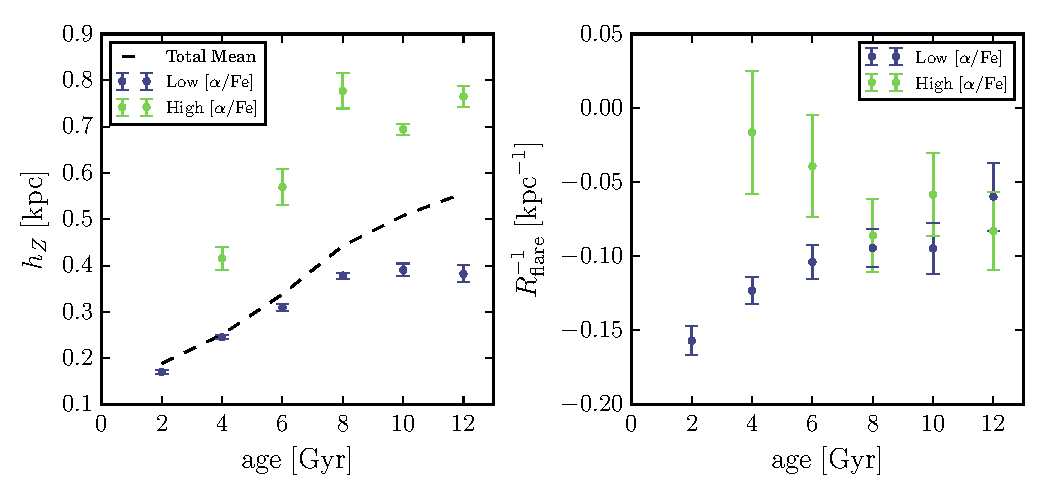
\includegraphics[width=\textwidth]{hzrfbroadvsage.pdf}
    \caption[$h_Z$ and $R_\mathrm{flare}^{-1}$ as a function of age for high and low-\afe{} mono-age populations in APOGEE DR12]{ Mean $h_Z$ at $R_0$ (\emph{left}) and $R_{\mathrm{flare}}^{-1}$ (\emph{right}) against age. The mean value in each age bin is calculated by multiplying together the posterior PDFs of the density fits. The panels show both the low (\emph{purple}) and high (\emph{green}) \afe{} populations. The left panel shows the total surface-mass density weighted mean as a dashed line, which demonstrates that the vertical distribution of the high-\afe{} population is only important at the solar radius at old ages due to its low surface-mass density contribution. $h_Z$ increases with age for both low and high-\afe{} populations. $R_{\mathrm{flare}}^{-1}$ behaves similarly for the low-\afe{} population, meaning flaring decreases with age, but the high-\afe{} population shows an opposite behaviour.}
     \label{fig:agevshzrf}
\end{figure}

\subsection{The mass contribution of mono-age, mono-\feh{} populations}
\label{sec:surfmassdens}
I now present the results from the calculation of the surface-mass density at the solar radius using the method described in Section \ref{sec:surfmasscalc}. The surface-mass density $\Sigma_{R_0}$ estimates are computed in each age-\feh{} bin in the high and low-\afe{} populations. When quoting the surface-mass densities, I also quote estimates of the systematic uncertainties. The sources of these uncertainties are evaluated and discussed in Section \ref{sec:discrepant}.

I combine the mass contributions of the high and low-\afe{} mono-age, mono-\feh{} populations, and plot these estimates as a function of age and \feh{} in Figure \ref{fig:margmass}. This Figure is representative of the \emph{mass-weighted} age-\feh{} distribution at the solar radius, i.e. it is equivalent to the probability distribution of age and \feh{} of a randomly selected mass element at the solar radius. The distribution varies smoothly with no sharp peaks, and the surface-mass density increases linearly with both age and \feh{}, peaking at $1 < \mathrm{age} < 3$ Gyr, $0.0 < \mathrm{[Fe/H]} < 0.1$ dex. The mass increases more smoothly with \feh{} than with age, but there is very little mass in the highest \feh{} bin, creating a ridge feature in the marginalised distribution. The distributions marginalised over age and \feh{} are clearly unimodal at this resolution, and there is little sign of any bimodality in age at fixed \feh{}. It should be mentioned again here that the age uncertainties may be larger than the bin width, particularly in older bins, which would cause an artificial blurring of a density edge in the distribution along the age axis. Therefore, one cannot presently determine to high significance that there are no discontinuities in this distribution.

\begin{figure}
 	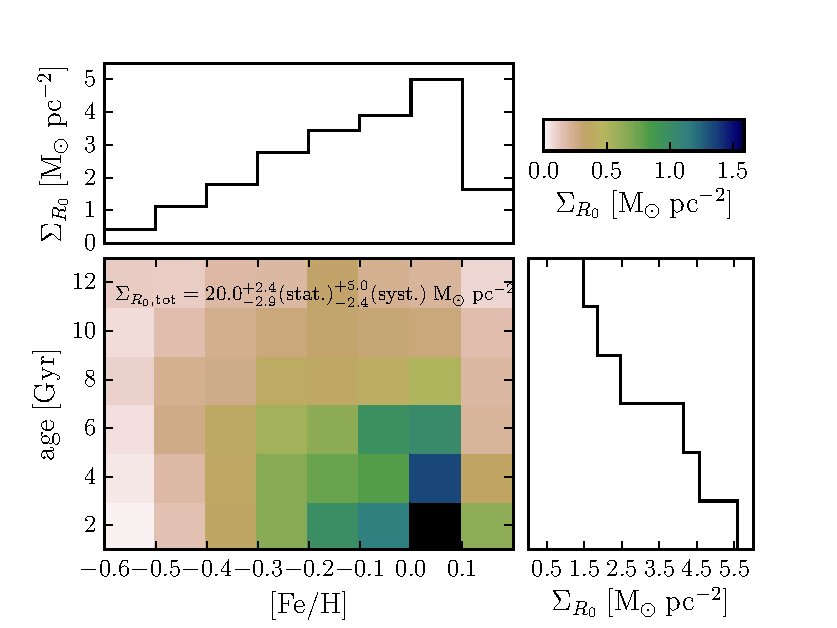
\includegraphics[width=\textwidth]{marginalised_colorblocks.pdf}
 	\centering
     \caption[The surface-mass density contribution of mono-age mono-\feh{} populations at the solar radius from APOGEE DR12]{The surface-mass density contribution of mono-age, mono-\feh{} populations at $R_0$ (where low and high-\afe{} are combined). The total contribution $\Sigma_{R_0,\ \mathrm{tot}}$ is displayed at the top of the main panel. The colour scale is linear and spans the surface-mass density range between $0 < \Sigma_{R_0} < 1.5\ \mathrm{M_{\odot}\ pc^{-2}}$. The marginalised distributions along each axis are shown above and to the right. The mass at the solar radius increases monotonically with both age and \feh{}. }
     \label{fig:margmass}
\end{figure}


An alternative way to look at the surface-mass density distributions is to retain the division in \afe{} used in the analysis. The high-\afe{} populations contribute $\Sigma_{R_0,\ \mathrm{tot}} = 3.0_{-0.5}^{+0.4}\mathrm{(stat.)}_{-0.6}^{+0.6}\mathrm{(syst.)}\ \mathrm{M_{\odot}\ pc^{-2}}$ to the total surface-mass density at the solar radius, whereas the low-\afe{} populations contribute $\Sigma_{R_0,\ \mathrm{tot}} = 17.1_{-2.4}^{+2.0}\mathrm{(stat.)}_{-1.9}^{+4.4}\mathrm{(syst.)}\ \mathrm{M_{\odot}\ pc^{-2}}$, giving a total surface-mass density in stars at $R_0$ of $\Sigma_{R_0,\ \mathrm{tot}} = 20.0_{-2.9}^{+2.4}\mathrm{(stat.)}_{-2.4}^{+5.0}\mathrm{(syst.)}\ \mathrm{M_{\odot}\ pc^{-2}}$. I plot the individual surface-mass contributions for the separated low and high-\afe{} populations in Figure \ref{fig:massafe}, adopting different color scales in each panel, to highlight the behaviour of the high-\afe{} populations, which contribute little mass in comparison to the low-\afe{}. The low-\afe{} mass is mostly concentrated at young age and towards higher \feh{}, although there is some mass even at the oldest ages. The high-\afe{} mass is concentrated towards older ages, but the distribution extends to high \feh{}, and mass is detected at some \feh{} in every age bin, albeit at much lower levels. The tails of the distributions of the low and high-\afe{} populations overlap somewhat in age-\feh{} space, around 6 Gyr ago, and there is a hint at the existence of a sequence extending from old, low \feh{} and high-\afe{} populations, to young, high \feh{} and low-\afe{} populations, which is somewhat visible in the combined histogram. There is no clear bimodality in age at fixed \feh{} in the combined histogram, owing to the very low mass contribution of the old, high-\afe{} populations. 

\begin{figure}
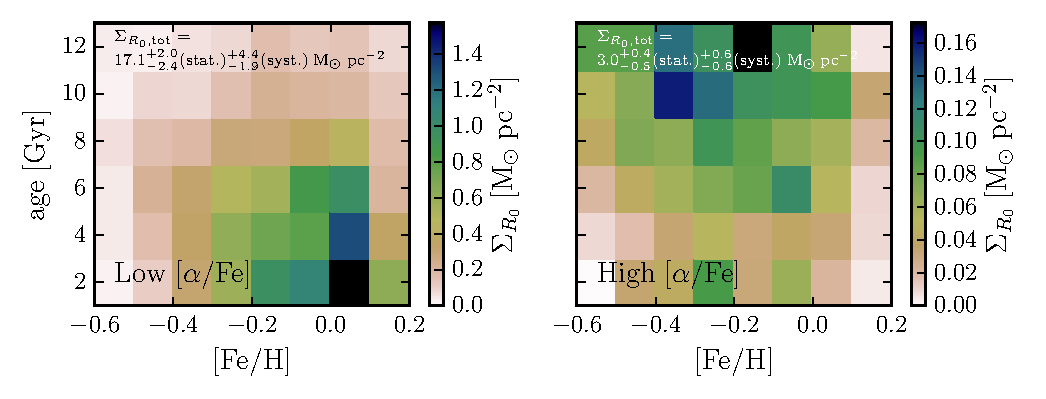
\includegraphics[width=\textwidth]{surfmassdensity_colourblocks_test.pdf}
 	\centering
     \caption[The separated surface mass density contributions of mono-age, mono-\feh{} populations in the low and high-\afe{} populations]{The surface-mass density contributions of the low (\emph{left}) and high (\emph{right}) \afe{} sub-samples. The total contributions $\Sigma_{R_0,\ \mathrm{tot}}$ are displayed at the top of each panel. I draw the attention of the reader to the difference in colour scale between the high and low-\afe{} panels, which differs by an order of magnitude, and is adopted to better show the behaviour in the high-\afe{} sample. The low-\afe{} sub-sample has mass at all ages and \feh{} but is concentrated mostly at young ages. The high-\afe{} sub-sample contributes far less mass and is concentrated at old age.}
     \label{fig:massafe}
\end{figure}


Thus far, I have established that the vertical spatial distributions of mono-age, mono-\feh{} populations are well described by single exponentials with a single characteristic $h_Z$. I now use this information to generate the mass-weighted distribution of $h_Z$, which is equivalent to the probability distribution function for $h_Z$, $p(h_Z)$. For a random stellar mass element, this function gives the probability density for the $h_Z$ of the component to which it belongs.  This relation is shown in Figure \ref{fig:hzhistogram}, where coloured points represent the individual density contributions of mono-age, mono-\feh{} populations, and the coloured histograms their co-addition within $\sim 0.1$ kpc wide bins in $h_Z$ for the low and high-\afe{} populations (purple and green, respectively). The dashed histogram represents the resulting total $p(h_Z)$. Scatter points are coloured by the age of the population they represent. The total distribution is smooth, resulting from the superposition of the low and high-\afe{} distributions, which overlap significantly.  The total $\Sigma_{R_0}$ (dashed histogram) declines exponentially with $h_Z$, and is unimodal with no gaps. The trends of both $h_Z$ and $\Sigma_{R_0}$ with age seen in Figures \ref{fig:agevshzrf} and \ref{fig:margmass} are recovered here, although it is surprising that the trend of $h_Z$ with age at the high $h_Z$ end does not appear as obvious here.

 \begin{figure}
	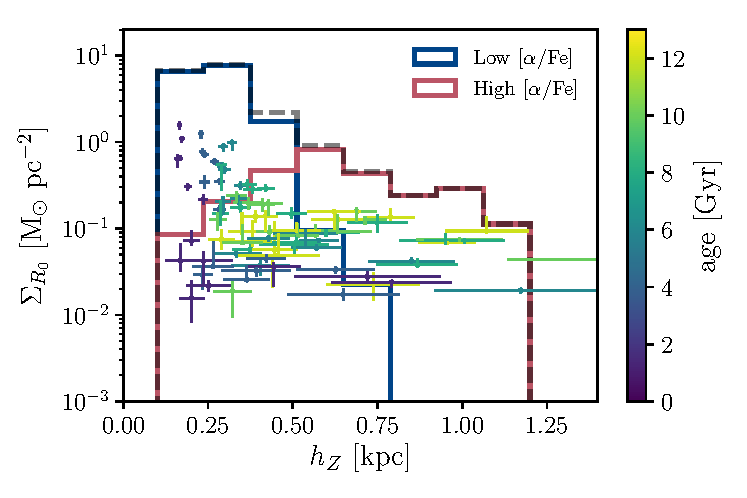
\includegraphics[width=\columnwidth]{thesis/Plots/adjusted_hz_sigma.pdf}
 	\centering
     \caption[The mass weighted vertical scale height distribution as calculated using mono-age, mono-\feh{} populations in APOGEE DR12]{The mass weighted vertical scale height $h_Z$ distribution. The individual points represent the $h_Z$ and $\Sigma_{R_0}$ for each mono-age, mono-\feh{} population. The points, which represent both the low and high-\afe{} populations, are coloured by the central age of the mono-age, mono-\feh{} bin that they represent. The coloured histograms represent the $h_Z$ distributions for the low and high-\afe{} populations from the sum of the individual contributions. The dashed histogram represents the total distribution. The total distribution smoothly decreases with $h_Z$, with no hints of bimodality.}
     \label{fig:hzhistogram}
 \end{figure}

I also now mass-weight and combine the fitted density profiles to attain the true surface-mass density profile of the Milky Way as a function of age, \feh{} and \afe{}. The resulting profiles are displayed in Figure \ref{fig:profcombo}. The different nature of the low and high-\afe{} populations in terms of spatial structure is clear here, with the low-\afe{} profile having a clear break between 8 and 10 kpc, and the high-\afe{} declining exponentially with $R$. It is interesting to note that extrapolation by eye of the high and low-\afe{} profiles to low $R$ would result in the high-\afe{} population becoming dominant over the low. The total profile appears roughly flat out to $\sim 10$ kpc. However, I \emph{strongly} emphasize that this is not determined to high significance, as even when only the uncertainties from the fitting procedure are included, one could describe the profile as exponentially declining with $R$ within $R < R_0$. The inclusion of the other sources of uncertainty on the surface-mass density estimates further decrease the significance of the apparent flattening. For example, the systematic uncertainties (discussed in Section \ref{sec:discrepant}) act to increase the fraction of surface-mass density contributed by the high-\afe{} populations, which would only \emph{increase} the slope of the inner exponential. Using dynamical tracers, \citet{2013ApJ...779..115B} find that the total surface density declines exponentially with R, so it seems logical to assume that the inner profile should not be increasing with R.

As a function of age, the peak in the surface-mass density visible in the youngest population becomes less prominent, and the profile becomes a roughly single exponential at the oldest ages (i.e., it monotonically decreases with $R$).  The behaviour with \feh{} is more complex, but the variation of the peak radius with \feh{} is obvious, and the turnover in the total profile at $\sim 10$ kpc appears to be a result of the outermost breaks.

\begin{figure}
 	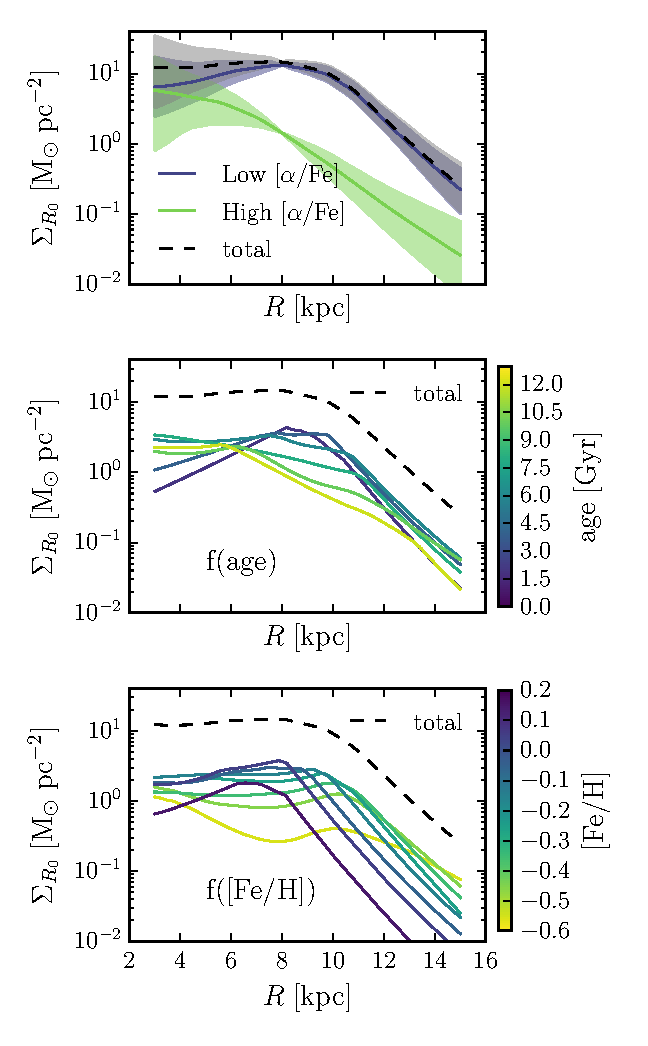
\includegraphics[width=0.7\columnwidth]{massweightedsurfdens.pdf}
 	\centering
     \caption[The best fit model for the true radial surface density profile of the Milky Way, as a function of age, \feh{} and \afe{} using mono-age mono-\feh{} populations in APOGEE DR12]{The radial surface-mass density profile of the Milky Way, as a function of \afe{} (\emph{top}), age (\emph{middle}) and \feh{} (\emph{bottom}). The profiles are the result of a mass-weighted combination of the fitted density profiles along different axes in age-\feh{} space and (in the top panel) for the combined low and high-\afe{} populations. Tthe combined uncertainties from the fitting procedure are shown in the top panel, which are sufficient (without addition of the individual statistical and systematic errors on the surface-mass densities, which are substantial) to show that the apparent flattening at $R < R_0$ is not found to high significance. The surface-mass density of low-\afe{} stars extends to a higher radius than the high-\afe{} stars. The youngest populations show a clearly peaked surface-mass density around the solar radius, whereas the older populations peak more centrally. Behaviour with \feh{} is complex, with flat profiles at low $R$, becoming exponentially decreasing at high $R$.}
    \label{fig:profcombo}
 \end{figure}

 \section{Discussion}
 \label{sec:discussiona}
 In the above analysis, I have, for the first time, determined the detailed structure of the Milky Way's disc as a function of stellar age and \feh{}. In our method, I have drawn heavily from previous dissections of the disc into its mono-abundance constituents \citep[MAPs;][]{2012ApJ...753..148B,2016ApJ...823...30B}, and so use these previous findings as a benchmark with which to compare these results. I will also show that our results are broadly consistent with other measurements, whilst shedding new light onto the problem of the formation of the Milky Way disc.


\subsection{Surface-mass density systematics}
\label{sec:discrepant}
I first address the sources of systematic uncertainty in our surface-mass density estimates, which are pertinent to the following discussions. The total local surface-mass density, including the correction for stars missing from the age catalogue, but before accounting for any other systematic uncertainties, is $\Sigma_{R_0, \text{tot}} = 20.0_{-2.9}^{+2.4}\ \mathrm{M_{\odot} \ pc^{-2}}$. This result is roughly two thirds as large as previous estimates, which are of the order $\Sigma_{R_0, \text{tot}} \sim 30\ \mathrm{M_{\odot} \ pc^{-2}}$ \citep[e.g.][]{2006MNRAS.372.1149F,2012ApJ...751..131B,2015ApJ...814...13M}. From canonical stellar evolution it is known that giants contribute very little to the total stellar mass in any population. For instance, \citet{2015ApJ...814...13M} find that giants make up $\sim 2\%$ of the local stellar mass. By virtue of this fact, conversions of the stellar mass inferred from giant-star counts to that of the total underlying stellar population require a multiplication of the observed counts by a factor of $\sim 50$, meaning that any uncertainty in the star counts is amplified in the final surface-mass density estimate. Our quoted statistical error estimates, however, which account for Poisson fluctuations in the stellar counts, cannot fully account for the discrepancy. 

I first evaluate whether such a discrepancy may be due to the assumed IMF or stellar evolution model. Tests adopting exponential \citet{2003PASP..115..763C} and \citet{2001MNRAS.322..231K} IMFs for the mass calculation resulted in variations of the final $\Sigma_{R_0, \text{tot}}$ estimate of the order $\sim 1\ \mathrm{M_{\odot}\ pc^{-2}}$, which I incorporate into the systematic error budget. I also re-ran the analysis on the basis of the BaSTI stellar evolution models \citep{2004ApJ...612..168P}, for which there also exists calculations for $\alpha$-enhanced stars \citep{2006ApJ...642..797P}. This test produces comparable estimates to the PARSEC models (after correcting for the fact that the lowest mass in the BaSTI isochrones is $0.5\  \mathrm{M_{\odot}}$ as opposed to $0.1\ \mathrm{M_{\odot}}$ in the PARSEC models). I also compute the mass using only APOGEE fields away from the plane (with $|b|\geq 6^{\circ}$), to test for the effects of extinction on the star counts, but attain results within the Poisson uncertainties of the original estimate.

I also apply our analysis procedure to a basic Monte Carlo mock sample, to check the method for converting observed counts to the real number density $N(R_0)$. I sample stars on a broken exponential density distribution with exponential flare then select points within APOGEE fields out to an imposed distance cut (which allows a simple reconstruction of the selection, and calculation of the effective volume). I then calculate $N(R_0)$ analytically, and also via our method, and find results which are consistent with the input parameters of the model, within the Poisson errors, for a wide variety of input parameters. 



As mentioned in Section \ref{sec:ages}, after making corrections to the ages, I find that the model returns ages greater than 13 Gyr for a sizeable number of stars \citep[][limit ages to 13 Gyr in their table]{2016MNRAS.456.3655M}. While these stars make up approximately $10\%$ of the final sample (3020 stars), they are not included in the number counts in each mono-age mono-\feh{} bin for calculation of the surface-mass density. Adding an extra $10\%$ of counts to each bin (in the same way as the extra $25\%$ is added in Section \ref{sec:ages}) introduces an extra systematic uncertainty of roughly $1\  \mathrm{M_{\odot}\ pc^{-2}}$ in each \afe{} sub-sample. However, readers should take into account that this simple correction does not account for a scenario where the stars with ages fitted $> 13$ Gyr might have a specific distribution in age, casting more counts in some bins (which might have more mass contribution per star) than others. For example, if these stars were all old, then the actual surface mass density in older bins would be higher than that found here, which would increase the total surface-mass density estimate. 

From the above, I robustly conclude that the majority of the systematic discrepancy is likely not due to the assumed IMF, stellar evolution model, dust extinction, or some peculiarity in the age measurements which affects star counts in the bins used. At this stage, it is difficult to understand what is the possible origin of this discrepancy with other works in the literature. Interestingly, this study is the only one employing giant stars as the stellar population tracer, which may point to possible systematics in the theoretical isochrones, or the APOGEE stellar parameters, or a combination thereof. It was demonstrated by \citet{2017A&A...597L...3M} that there may be significant issues with the spectroscopic determination of stellar surface gravity, which is dependent on the star's evolutionary state. I do find some discrepancy between the $\log{g}$ of the red clump between the PARSEC isochrones and the data, of the order $\sim 0.2$ to $0.3$ dex \citep[similar to that found by][albeit based on APOGEE-DR13 data]{2017A&A...597L...3M}, which could conceivably lead to problems in the conversion between star counts and mass. 

I test for the effect of systematics in the $\log{g}$ scale by shifting the $\log{g}$ cut of the isochrones to lower and higher $\log{g}$ by $0.3$ dex. I find that shifting the $\log{g}$ cut by $-0.3$ dex increases the surface-mass density estimate by $5.0\ \mathrm{M_{\odot}\ pc^{-2}}$. Increasing the $\log{g}$ cut by $0.3$ dex results in a decrease of $ 2.4\ \mathrm{M_{\odot}\ pc^{-2}}$. It therefore seems plausible that the discrepancy results from a systematic difference between the $\log{g}$ scales of the theoretical isochrones and APOGEE, and so I incorporate these shifts into the systematic error estimate. 

Upon inclusion of the systematic uncertainties from IMF variations and differences in the surface gravity scales, a final estimate of the total local surface-mass density in visible stars of $\Sigma_{R_0, \text{tot}} = 20.0_{-2.9}^{+2.4}\mathrm{(stat.)}_{-2.4}^{+5.0}\mathrm{(syst.)}\ \mathrm{M_{\odot} \ pc^{-2}}$, is attained from the addition of the low-\afe{} surface-mass density of $\Sigma_{R_0, \text{tot}} = 17.1_{-2.4}^{+2.0}\mathrm{(stat.)}_{-1.9}^{+4.4}\mathrm{(syst.)}\ \mathrm{M_{\odot} \ pc^{-2}}$, and the high-\afe{} value of $\Sigma_{R_0, \text{tot}} = 3.0_{-0.5}^{+0.4}\mathrm{(stat.)}_{-0.6}^{+0.6}\mathrm{(syst.)}\ \mathrm{M_{\odot} \ pc^{-2}}$.  If the $\log{g}$ systematics are as large as $-0.3$ dex, then this result is in agreement with the recent estimate from \citet{2015ApJ...814...13M}, of $27\pm 2.7\ \mathrm{M_{\odot} \ pc^{-2}}$.

A recent compilation of measurements of the thick and thin discs found that the thick-thin disc surface density ratio at $R_0$ is $f_{\Sigma} = 15\% \pm 6\%$ \citep{2016ARA&A..54..529B}. I find that $f_{\Sigma} = 18\% \pm 5\%$ for the high-low-\afe{} disc surface-mass density ratio, consistent with that estimate. While a better understanding of the possible systematics between the theoretical isochrones and APOGEE is beyond the scope of this paper, I have shown that even a slight difference in the $\log{g}$ scale can bring our results in line with existing estimates. This suggests that the surface-mass density measurement discrepancy here is indeed systematic, and that the high and low-\afe{} discs may still have some relation to the thick and thin components measured by these studies, which are mainly based on geometric decompositions of the disc. 

\subsection{Comparison with MAPs results}
\label{sec:bovycomparison}
I now discuss our density fits in comparison to the MAP measurements of \citet{2012ApJ...753..148B,2016ApJ...823...30B}. Such a comparison is important because this method is based on an extension of that developed by \citet{2016ApJ...823...30B} to the case of RGB stars, whose distances are far more uncertain than those of RC stars. \citet{2016ApJ...823...30B} used the APOGEE RC sample to find the structure of populations in narrow bins of \afe{} and \feh{}, which they term `mono-abundance populations' (MAPs). These MAPs represent stellar populations with a distribution of ages, but their interpretation assumes a significant relationship between age, \afe{} and \feh{}. I can now compare results when the third parameter, age, is known.  

\citet{2016ApJ...823...30B} showed that the radial distribution of low-\afe{} MAPs is well described by a broken exponential, and I confirm this result, showing that each of the low-\afe{}, mono-age, mono-metallicity populations is also described by a radially broken exponential. I also show that the older, high-\afe{} populations are instead described by a single exponential, which is in good agreement with the findings of \citet{2016ApJ...823...30B}.

The dependence of the radial distribution of mono-\feh{} populations on age is interesting in this regard.  The low-\afe{} population, for which our sample covers a wide range of ages with high signal-to-noise, shows a broadening of the profile around a density peak towards older populations, at all \feh{}. This effect does not appear to be present in the high-\afe{} population (although some populations have slight evidence of a break at low significance), which suggests that it was formed and evolved differently. The implications of these findings are more fully discussed in Section \ref{sec:implications}.

I also confirm the results of \citet{2016ApJ...823...30B} which showed that the break radius, $R_{\mathrm{peak}}$ is a declining function of \feh{}. I show that, in the low-\afe{} population, at fixed age, $R_{\mathrm{peak}}$ moves to smaller radii as \feh{} increases. As a function of age, the amplitude of this variation increases. The difference in $R_{\mathrm{peak}}$ at the highest and lowest \feh{} in the 6 Gyr bin is $\sim 6$ kpc, which is identical with that of the profiles shown in Figure 11 of \citet{2016ApJ...823...30B}.
 
\citet{2016ApJ...823...30B} found that low-\afe{} MAPs were fit well with a $h_Z(R)$ which was slowly exponentially flaring with $R_{\mathrm{flare}}^{-1} = -0.12 \pm 0.01 \ \mathrm{kpc^{-1}}$. I also confirm this result, finding that low-\afe{} populations have, on average, $R_{\mathrm{flare}}^{-1} = -0.12 \pm 0.01 \ \mathrm{kpc^{-1}}$. However, I also find that $R_{\mathrm{flare}}^{-1}$ shows considerable variation with age (around this mean) in the low-\afe{} populations. While \citet{2016ApJ...823...30B} found that high-\afe{} populations were consistent with a having $R_{\mathrm{flare}}^{-1} = 0.0 \pm 0.02\ \mathrm{kpc^{-1}}$, I find that these populations have $R_{\mathrm{flare}}^{-1} = -0.06 \pm 0.02\ \mathrm{kpc^{-1}}$, showing some evidence of flaring, albeit at a lower level and lower significance than the low-\afe{} populations.

 It was also shown by \citet{2012ApJ...753..148B,2016ApJ...823...30B} that the $h_Z$(\afe{},\feh{}) of MAPs smoothly spans the range between 0.2 and 1 kpc. I confirm and extend this result, showing that $h_Z$(age,\afe{},\feh{}) varies smoothly between a maximum $h_Z$ of $\sim 1.2$ kpc in the high-\afe{}, low \feh{}, older populations, down to a minimum of $\sim 0.2$ kpc in the youngest, low-\afe{}, \feh{} rich populations. Figure \ref{fig:hzhistogram} can also be directly compared with Figure 2 of \citet{2012ApJ...751..131B}, which showed that the mass-weighted $h_Z$ distribution is not bimodal but smoothly declines with $h_Z$. I confirm that result, showing that for mono-age, mono-metallicity populations, the mass weighted $h_Z$ distribution shows no sign of bimodality; The low and high-\afe{} population $h_Z$ distributions are distinct but overlap significantly, generating a smooth distribution. This presents an interesting new look at the interplay between spatial and chemical structure in the disc, as there is a clear mixing spatially of the two chemically separated populations. The implications of this finding are intriguing, and I discuss them further in Section \ref{sec:implications}.

\citet{2012ApJ...751..131B} also made a measurement of the local surface-mass density, finding (in the original application of the method used here) that SEGUE G-type dwarfs yield an estimate of $\Sigma_{R_0,\text{tot}} = 30 \pm 1\ \mathrm{M_{\odot}\ pc^{-2}}$, which is in good agreement with other studies based on different samples \citep[e.g.][]{2006MNRAS.372.1149F,2015ApJ...814...13M}.  Comparatively, the estimate based on APOGEE DR12 somewhat smaller, even when systematics are taken into account. There are a number of differences between this study and that of \citet{2012ApJ...751..131B}. For example, the increased radial coverage, adoption of RGB stars as a tracer, and the fits based on mono-age, mono-metallicity (rather than mono-abundance) populations. However, as mentioned above in Section \ref{sec:discrepant}, these results, after accounting for systematic uncertainties, appear in good agreement with other, more recent estimates \citep{2015ApJ...814...13M}. 

\subsection{Comparison with other Milky Way disc studies}
I now make qualitative comparisons of the findings of this analysis with the broader body of knowledge regarding the Milky Way disc structure \citep[see, e.g.][for recent reviews]{2013A&ARv..21...61R,2016ARA&A..54..529B}. In comparing these results with those from previous studies, I am constrained to making mostly qualitative considerations, as previous work is based on fits of single exponential profiles to the radial component of the stellar density distribution.

This work strongly constrains the structure of both the low and high-\afe{} components in the Galactic disc, which are commonly considered to be interchangeable with the thin and thick components \citep[as asserted by, e.g.][]{2004A&A...415..155B,2012A&A...545A..32A,1998A&A...338..161F}. I have shown that the \afe{} rich component, while corresponding to a thicker configuration in general, is the product of individual mono-age populations of varying thickness. I also find that the \afe{} rich populations span the range  $ 0.4 < h_Z < 1$ kpc, with $h_Z$ increasing with age. Studies of the vertical disc structure which fit a double exponential find a thick disc scale height of $\sim 1$ kpc  \citep[e.g.][]{1983MNRAS.202.1025G,2008ApJ...673..864J}, which is fully consistent with measurements of the thickest high-\afe{}, old, mono-age populations in our analysis. However, I again stress here that the age uncertainties at old ages may be significantly larger than the bin size, which may cause a blurring of these trends, and should be accounted for when comparing these results to models. As an example, in the \emph{worst case} scenario, assuming gaussian errors, the oldest bins (between 7 and 13 Gyr) may be contaminated by up to $50\%$ of the stars which should be assigned to neighbouring bins, at the oldest end, with the fraction dropping off quickly at younger ages. I briefly discuss the implications of the worst case blurring on our interpretation of these trends in Appendix \ref{sec:ageerror}.

Regarding the radial scale length of the thick component, I find an obvious discrepancy with literature values, whereby our thick, high-\afe{}, populations have an average $h_{R, \text{out}} = 1.9 \pm 0.1  $ kpc, while the aforementioned studies, who define the thick disc geometrically, find values of the order $\sim 4$ kpc \citep{2001MNRAS.322..426O,2008ApJ...673..864J}. This discrepancy appears to arise in the choice of definition of the measured population between a geometric or chemical abundance selection, with many studies finding a scale length for the abundance-selected $\alpha$-rich disc in the range $h_R = 2.0 \pm 0.2$ kpc \citep{2016ARA&A..54..529B,2016ApJ...823...30B,2012ApJ...753..148B,2012ApJ...752...51C}. It should be noted here that the $h_{R, \text{out}}$ found here would likely be in even better agreement with this value, had the 5\% systematic discrepancy in the distances (shown in Figure \ref{fig:distcomp}) been accounted for. \citet{2016arXiv160901168M} recently showed evidence for a radial age gradient in the Milky Way, suggesting this as a source of disagreement between abundance-selected and geometric studies of the thick disc components, where the geometric selected studies see an extended thick disc which is made up of flared low-\afe{} populations. 

I also re-examine claims of a sharp decline in the stellar density at $R\sim 13.5$ kpc \citep[e.g.][]{2009A&A...495..819R,2010MNRAS.402..713S} in light of these results. \citet{2010MNRAS.402..713S} fit a single exponential density profile with scale-length $\sim 3$ kpc to A stars (which preferentially selects stars younger than $\sim 100$ Myr old) and found that after $R\sim13$ kpc, a model with shorter scale-length was necessary to explain the increased rate of decline in stellar density. The total profile in Figure \ref{fig:profcombo} begins to decline after $R\sim10$ kpc. The uncertainties in the measurement of the mass contribution of each profile may cause some discrepancy here, as implying a higher mass on older or more metal poor populations would shift this turn-over to higher radii. I also fit older populations than \citet{2010MNRAS.402..713S}, which, under the inside-out formation paradigm, might suggest another reason for such a discrepancy, as older populations would be more centrally concentrated. I confirm the assertion of \citet{2016ApJ...823...30B} that this break, clearly visible in the total stellar distribution, is attributable to the outermost break of the mono-\feh{} profiles - which are shown in the bottom panel of Figure \ref{fig:profcombo}. External disc galaxies are also observed to have such a truncation in their stellar density profiles \citep[e.g.][]{2006A&A...454..759P}. 


\subsection{Implications for the formation of the Galactic disc}
\label{sec:implications}

In light of the above discussion, I now present the implications of these results for the formation of the Galactic disc. In this chapter, I present a detailed dissection of the disc by age, \feh{}, and \afe{}, and as such, present a previously unseen picture of the dominant structure of the Milky Way. In studying mono-age populations, I enable a more direct comparison than previously possible with numerical simulations of Milky Way type galaxies, which tend to use age information in the absence of detailed chemical modelling.

\subsubsection{Disc flaring, profile broadening and radial migration}

By estimating the density profiles of mono-age populations, I  place novel constraints on radial migration and its effects on the structure and evolution of the disc. I describe two key observables which provide this insight: the flaring of the disc, which has been considered as an effect of vertical action conserving radial migration \citep[where stars have greater vertical excursions as they migrate outward, e.g.][]{2012A&A...548A.127M}, and the broadening of the density profiles around the peak with time, which I discuss as a potential new indicator of radial migration. The right panel of Figure \ref{fig:agevshzrf} shows a clear trend of increasing $R_{\mathrm{flare}}^{-1}$ with age such that the youngest populations flare most. This behaviour is distinct from the results of \citet{2016ApJ...823...30B}, which found that low-\afe{} populations were described by a single $R_{\mathrm{flare}}^{-1}$. It is, however, conceivable that if low-\afe{} populations of all ages are combined, the resulting population may have a similar behaviour to that in \citet{2016ApJ...823...30B}. Indeed, I find an average $R_{\mathrm{flare}}^{-1} = -0.12\pm 0.01\ \mathrm{kpc^{-1}}$, which is in good agreement with the value from \citet{2016ApJ...823...30B}. If populations become more flared as radial migration proceeds, then it becomes difficult to reconcile our result with that of a disc whose stars continually underwent radial migration, largely unperturbed by any mergers that might cause structural discontinuity \citep[e.g.][]{2014MNRAS.442.2474M}, especially under suggestions that mergers actually reduce flaring from radial migration \citep[e.g.][]{2014A&A...572A..92M}. In this context, this result is indicative of an old population in the Milky Way which has undergone some mergers, reducing the flaring in the oldest populations. It should be noted here, however, that the age uncertainties (which can be as large as $40\%$) could effectively artificially increase the age bin size, super-imposing populations with different scale heights and flare, and reducing the overall flaring profile.

I show in Figures \ref{fig:agevsbroadening} and \ref{fig:surfdens}  that the radial surface density profiles of low-\afe{} populations become smoother with age. Interestingly, the position of the break radius does not vary monotonically with age. Assuming that the peak radius is at the equilibrium point of chemical evolution for a given population  \citep[where the consumption of gas and its dilution are balanced, as discussed in][]{2016ApJ...823...30B}, then one might consider that such a broadening would occur if stars that formed near the equilibrium point migrated inwards and outwards over time.  If these assumptions are correct, then the specific surface density profile shapes might provide insights into how radial migration has proceeded in the disc. For example, if the slope of the inner or outer profile change slope differently, this might suggest that migration has been asymmetric (i.e. more mass has moved in than out or vice versa). Comparing the $-0.2 <\mathrm{[Fe/H]}<-0.1$ dex and $0.0 <\mathrm{[Fe/H]}<0.1$ dex bins in Figure \ref{fig:surfdens}, it seems that the \emph{inner} slope of the former profile decreases more with age, whereas the \emph{outer} slope of the latter decreases more strongly, suggesting that the former population has preferentially migrated in, whereas the latter migrated out.  It is important to point out that under the interpretation that the increasing profile width is due to migration efficiency, I make an assumption that stars of a given \feh{} and \afe{} must have been born with the same profile width throughout cosmic time \citep[as discussed by, e.g.][]{2017ApJ...834...27M}.


This picture is also consistent with the suggestion by, e.g, \citet[][]{2015ApJ...808..132H,2011ApJ...737....8L}, that the changing skew in the MDF as a function of Galactocentric radius is caused by such a mechanism. In Figure \ref{fig:mdf}, I show the mass-weighted \feh{} distribution for the low-\afe{} fits at different Galactocentric radii, showing that these results both find a radial metallicity gradient, and qualitatively reproduce the skew found by \citet[][]{2015ApJ...808..132H}. Unlike \citet[][]{2015ApJ...808..132H}, this analysis fully corrects for sample-selection and stellar-population biases in reconstructing the MDF. \citet{2016MNRAS.460L..94G} also found similar behaviour in a simulated galaxy, finding that spiral structure induces different migration patterns, dependent on birth radius. 

\begin{figure}
	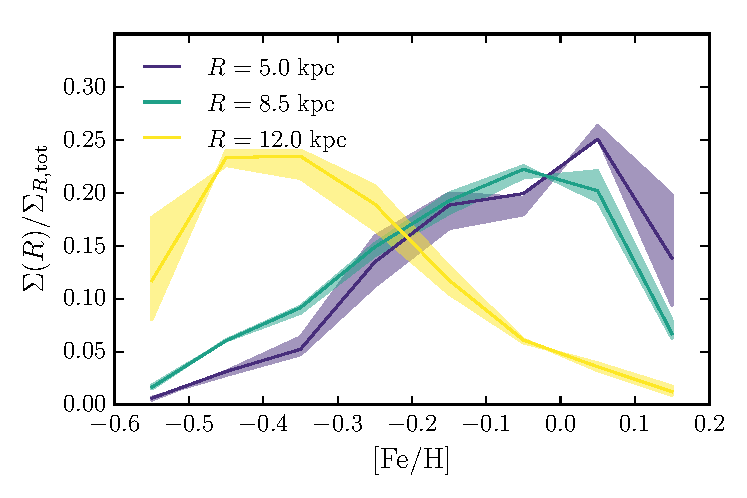
\includegraphics[width=0.8\columnwidth]{MDFs_radii.pdf}
 	\centering
   \caption[Surface-mass denisty weighted \feh{} distribution in 3 radial bins, as found from measurement of mono-age, mono-\feh{} populations in APOGEE DR12]{The surface-mass density weighted \feh{} distribution (MDF) at 3 radii for profiles fit to the low-\afe{} populations. The distribution shown is marginalised in age across all age bins. The coloured bands give the 95\% uncertainty ranges, where uncertainties are dominated by those on the fitted density profiles. The mean \feh{} is lower at greater $R$. Qualitatively, the skew of the MDF's changes with $R$, such that the innermost $R$ has a tail going to low \feh{}, and the outermost $R$ has a tail going to high \feh{}}
     \label{fig:mdf}
 \end{figure}

Interestingly, I detect the possible flaring of old, high-\afe{} populations, with average $R_{\mathrm{flare}}^{-1} = -0.06 \pm 0.02\ \mathrm{kpc^{-1}}$. However, the right panel of Figure \ref{fig:agevshzrf} shows that the flaring of the high-\afe{} populations does not vary as strongly with age as the low-\afe{} populations (although it should be noted that most of the mass in the high-\afe{} populations is concentrated at older age anyway). The detection of even a slight flare in these populations is surprising, as \citet{2016ApJ...823...30B} found that the high-\afe{} MAPs did not have any flare. Again, this may be an effect of the superposition of multiple mono-age populations within the MAPs. For example, \citet{2015ApJ...804L...9M} found that co-eval populations in simulated galaxies always flare, and suggested that the superposition of such flares might be an explanation for thickened disc components. \citet{2017ApJ...834...27M} showed that the superposition of mono-age populations within MAPs can introduce decreased flaring in high-\afe{} populations, whilst the mono-age populations themselves still flare. Comparison of these results with \citet{2016ApJ...823...30B} seems to present a consistent scenario. It should be noted here however, that \citet{2013MNRAS.436..625S} found that MAPs in their simulation were coeval in general.

These results show that the oldest populations are thicker, centrally concentrated, and display the least flaring, whilst the youngest populations, which show the most flaring, have the thinnest vertical distribution (smallest $h_Z$). Between these extremes, consecutive populations in age form a continuum, when the combined low and high-\afe{} structure is considered (see Figure \ref{fig:agevshzrf}). It is clearly conceivable then, that the \emph{geometrically} defined thick disc, found to have large scale-length \citep[e.g.,][]{2013MNRAS.431..930J,2008ApJ...673..864J}, may be the superposition of these flared (young) and naturally thick (old) components. An obvious consequence of this scenario would be an age-gradient at high $Z$ above the disc plane, which has been recently shown to be present in the APOGEE data by \citet{2016arXiv160901168M}. It was also recently shown that the mean structural characteristics of the abundance selected thick and thin discs appear to overlap at $\mathrm{[M/H]}\sim-0.25$ dex and \afe{} $\sim 0.1$ dex in the Gaia-ESO dataset \citep{2014A&A...567A...5R}, further presenting a scenario where the thick and thin disc components are not necessarily separable from one another, or at least not in abundance space. 

\subsubsection{Inside out formation, and the overall vertical disc structure}
The formation of the Galactic disc is commonly framed in the paradigm of inside-out formation \citep[e.g.,][]{2013ApJ...773...43B,2011ApJ...729...16K,1976MNRAS.176...31L,1989MNRAS.239..885M}. More recently, the effects of radial migration  \citep[e.g.][]{2002MNRAS.336..785S} were added, in order to produce models that agree better with the observations \citep[e.g.][]{2011ApJ...737....8L,2009MNRAS.396..203S,2015ApJ...802..129S,2015A&A...580A.126K} . The measurements of the peak radius of mono-age populations  presented in this chapter place strong empirical constraints on the evolution of the Milky Way disc over time. The behaviour of $R_{\mathrm{peak}}$ with age and \feh{} is shown in Figure \ref{fig:rpeakvsage}. I find that the surface-mass density weighted mean $R_{\mathrm{peak}}$ of low-\afe{} populations remains roughly constant with age, whilst the dispersion about the mean increases with age. This finding is qualitatively consistent with that of e.g. \citet{2016arXiv160804951A}, who show that the radial metallicity gradient decreases with the age of the population considered. These results show that the density peaks of mono-\feh{} populations become more separated with age. As the mean \feh{} at a given $R$ is dictated by the dominant population in stellar density at that radius, this indicates that these results also find a shallowing gradient in \feh{} with age. This is reinforced by our finding (also shown in Figure \ref{fig:rpeakvsage}) that the mean $R_{\mathrm{peak}}$ decreases with \feh{}.

\begin{figure}
	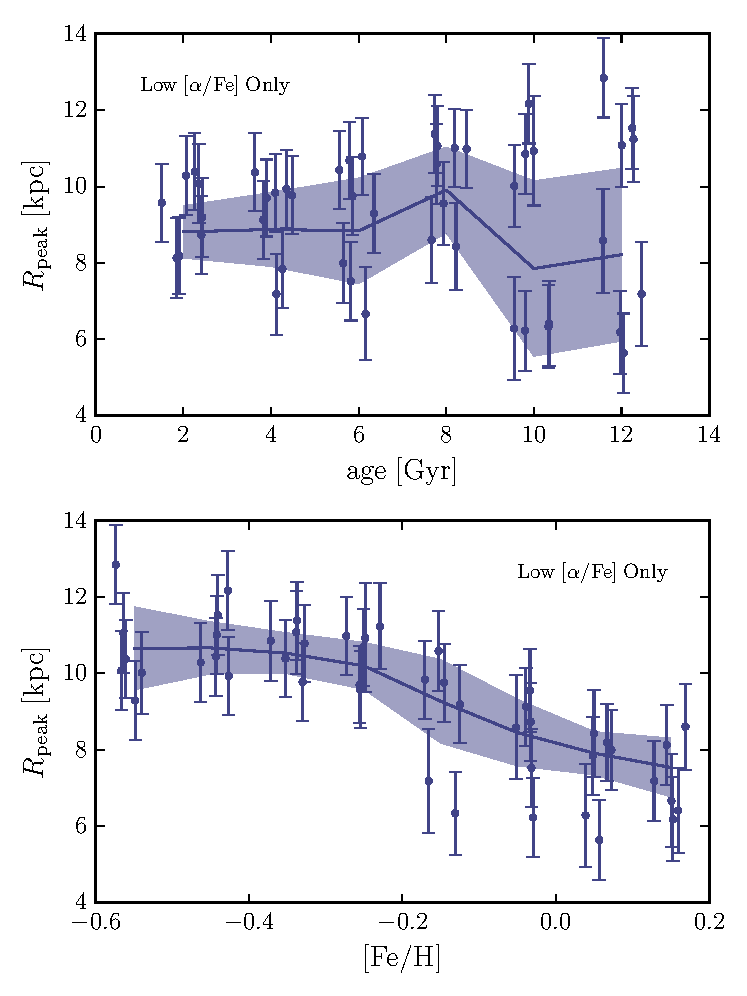
\includegraphics[width=0.8\columnwidth]{rpeakvsage.pdf}
	\centering
   \caption[Peak radius of surface density profiles in the low-\afe{} mono-age, mono-\feh{} populations in APOGEE DR12, shown as a function of age and \feh{}]{The behaviour of $R_{\mathrm{peak}}$ with age and \feh{} for the low-\afe{} populations. The high-\afe{} populations are better fit by single exponentials, and so $R_{\mathrm{peak}}$ is not an informative diagnostic of these populations. The coloured lines and bands give the surface-mass density weighted mean and standard deviation within an age or \feh{} bin. The mean $R_{\mathrm{peak}}$ does not vary significantly with age, whereas it shows a clear decrease with \feh{}. However, the dispersion in $R_{\mathrm{peak}}$ does increase with age for low-\afe{} populations. high-\afe{} populations show a slight increasing trend for increasing age and \feh{}, albeit at low significance. }
    \label{fig:rpeakvsage}
 \end{figure}


These results also place strong constraints on models for the formation of the vertical disc structure. I have already discussed that the vertical structure of the disc is commonly framed as having two geometrically distinct (but overlapping) vertical components \citep[e.g.][]{1983MNRAS.202.1025G}. The results of this chapter confirm previous work \citep[e.g.][]{2012ApJ...751..131B} which shows that this picture, while providing an acceptable description of the data when analysing the whole population, is not complete when individual populations, either abundance- or age-selected, are considered. I have shown (in Figure \ref{fig:hzhistogram}) that for a random mass element, the probability that it belongs to a population of a given $h_Z$ exponentially declines as $h_Z$ increases. There are no apparent breaks in this relation at the resolution which it is measured here, strongly suggesting that the spatial vertical disc structure is continuous. This finding, in stark contrast to the distinct discontinuities seen in the chemical structure of the entire disc \citep[e.g][]{2014ApJ...796...38N,2015ApJ...808..132H}, presents an interesting conundrum for galaxy formation theory. How is it possible that the \emph{spatial} structure of the disc be smooth and continuous, whilst the \emph{chemical} structure portrays a clear discontinuity?

Theoretical studies have, thus far, presented some clues as to how galaxy discs such as that of the Milky Way might form. As most studies fit single exponential radial profiles to simulated discs, quantitative comparisons are difficult, yet qualitative considerations can be made. \citet{2013MNRAS.436..625S} used a maximum likelihood method similar to \citet{2012ApJ...753..148B} to fit density profiles to MAPs in a simulated galaxy and found a continuous distribution of scale heights, but also found that their simulation showed a strongly geometrically distinct thick disc component. \citet{2013ApJ...773...43B} made detailed measurements of the mono-age populations in a high-resolution hydrodynamic Milky Way-like galaxy simulation, and found, similarly to these results that their scale heights gradually decreased with time, while the scale lengths increased, with populations forming thick and retaining that thickness in an 'upside-down and inside-out' disc formation. These results also find evidence of flaring in the thick components (as discussed in Section \ref{sec:bovycomparison}), which may point towards some structural evolution (via a process such as radial migration) after their formation. However, work on simulations by \citet{2009ApJ...707L...1B}  suggests early, turbulent gas as the origin for thicker disc components. A flare in the gas disc of the Milky Way, associated with the stellar component, is also observed in numerous studies \citep[e.g.][]{2014Natur.509..342F,2014ApJ...794...90K,1963SvA.....6..658L}, suggesting a formation of the disc with structural parameters similar to its progenitor gas disc.
 
\subsubsection{The age-\feh{} distribution and the evolution of the disc}
I now discuss how the present day structural parameters, in combination with the emergent picture of the mass distribution in age-\feh{} space at the solar radius, might offer deeper insights into the formation and evolution of the disc. 

I find, as may be expected, that the high-\afe{} populations contribute the majority of their mass at the solar radius at ages older than $\sim 6$ Gyr, although the mass contribution by old stars is extremely low compared to the younger populations. The middle panel of Figure \ref{fig:profcombo} shows that, if the populations follow the density models that I have fit, then the older stars become more dominant closer to the Galactic centre, which is suggestive of a weak mean radial age gradient, in qualitative agreement with theoretical predictions \citep[e.g.][]{2015ApJ...804L...9M} and observations of the thick disc \citep[e.g.][]{2016arXiv160901168M}. It is therefore not surprising that the bottom panel of Figure \ref{fig:profcombo} shows a clear variation in mean metallicity, in agreement with findings in other works \citep[e.g.][]{2012ApJ...746..149C,2016arXiv160804951A,2015ApJ...808..132H}. Only with high resolution hydrodynamical simulations, which accurately reproduce the stellar populations in galaxies, will it be possible to reconstruct the right combination of star formation history and radial mixing that led to these age and metallicity gradients, to gain a better understanding of the details of their formation.

In Figure \ref{fig:massafe}, an overlap in age-\feh{} space is visible between the high and low-\afe{} populations. While there appears to be mass at many \feh{} bins in the old populations, the overlap in age occurs at intermediate \feh{} at the solar radius. Previous studies have found that the youngest stars in the high-\afe{} sequence overlap in age with the oldest and most \feh{} poor stars in the low-\afe{} population \citep[e.g.][]{2013A&A...560A.109H}, and these findings appear to be consistent with that result. It should however, be noted, that at least some of this overlap is likely caused by the age uncertainties, which can be as high as 40\%. If the low-\afe{} population emerged from the remnants of the high-\afe{}, then it is likely that some sort of infall event must have occurred to return the ISM to low \feh{} and low-\afe{} before forming those stars \citep[as expressed by, e.g.,][]{1997ApJ...477..765C}. These scenarios are also discussed in the context of the APOGEE results by \citet{2014ApJ...796...38N}. To fully understand this, however, we will likely require a chemodynamical model which reproduces the bimodality in \afe{} at fixed \feh{}.

\section{Conclusions}
\label{sec:conclusionsa}

I have performed the first detailed dissection of the stellar populations of the Milky Way disc in age, \feh{} and \afe{} space, bridging the gap between the detailed observational understanding of mono-abundance populations \citep[e.g.][]{2012ApJ...753..148B,2016ApJ...823...30B} and the plethora of studies of co-eval stellar populations in simulated galaxies \citep[e.g][]{2013ApJ...773...43B,2014MNRAS.442.2474M,2013MNRAS.436..625S}. I have placed novel constraints on models for the formation of the Milky Way disc by combining detailed density models fit to the mono-age, mono-\feh{} populations of the low and high-\afe{} disc, with surface mass density contributions calculated on the basis of these density fits and stellar evolution models. I summarise the key results of this chapter as follows:
\begin{itemize}
\item \textbf{Radial and vertical profiles} The mono-age, mono-\feh{} populations of the \afe{} poor disc are well fit by a radially broken exponential, with a peak radius, $R_{\mathrm{peak}}$, that varies as a function of age and \feh{}. The distance between $R_{\mathrm{peak}}$'s of the low and high \feh{} populations increases with age, which I interpret as evidence for a decreasing \feh{} gradient with time \citep[e.g][]{2016arXiv160804951A}. The radial variation of the stellar surface density of the high-\afe{} mono-age populations is found to have insignificant breaks, and they are better fit by a single exponential in this disc region. As these populations are the oldest, this may be a sign of the disc evolution washing out the density peak over time, or may point to a different formation scenario for high-\afe{} stars, where no density peak ever existed. These findings are in good agreement with earlier studies of MAPs \citep{2016ApJ...823...30B}. I measure an average high-\afe{} population scale length of $h_{R,\text{in}} = 1.9 \pm 0.1$ kpc, and find scale heights between 600 and 1000 pc, in good agreement with current measures of the \afe{} rich disc scale length and height \citep[e.g. those outlined in][]{2016ARA&A..54..529B}. 
\item \textbf{Profile Broadening}  The radial surface density profile of the low-\afe{} populations broadens with age in a given \feh{} bin, which I interpret as evidence of the gradual dispersal of mono-\feh{} populations, presumably due to radial migration and radial heating. The variation in shape of the broken exponential profile changes differently depending on the population \feh{}, with \emph{low} \feh{} populations \emph{inner} profiles flattening faster, whereas the \emph{high} \feh{} \emph{outer} profiles flatten faster. I interpret this effect as tentative evidence for \feh{} dependent radial migration arising from pre-existing \feh{} gradients in the star forming disc. These results qualitatively reproduce those of \citet{2015ApJ...808..132H}, finding a skewed MDF that varies as a function of R.
\item \textbf{Flaring} Flaring seems to be present in almost all mono-age populations, at differing levels. I have shown that the inverse flaring scale length $R_{\mathrm{flare}}^{-1}$ increases with age, meaning that the youngest populations flare most strongly. This finding appears inconsistent with that above, under the assumption that flaring is the result of radial migration. However, these results may be reconciled by invoking a more active accretion history in the early life of the disc, which could have suppressed flaring \citep[e.g.][]{2014ApJ...781L..20M}.
\item \textbf{The surface-mass density at $R_0$} The total surface mass density at the solar radius is found to be  $\Sigma_{R_0, \text{tot}} = 20.0_{-2.9}^{+2.4}\mathrm{(stat.)}_{-2.4}^{+5.0}\mathrm{(syst.)}\ \mathrm{M_{\odot} \ pc^{-2}}$. Before allowing for systematics, this value is less than current estimates \citep[e.g.][]{2012ApJ...751..131B,2006MNRAS.372.1149F,2015ApJ...814...13M}, however, the systematic uncertainties are large, mainly due to a mismatch between the $\log{g}$ scales in APOGEE and the PARSEC models, and as such, I find our value to be consistent within the uncertainties. The relative contribution of high to low-\afe{} populations, $f_\Sigma$, is $18\% \pm 5\%$, which is consistent with existing measurements \citep[e.g.][]{2016ARA&A..54..529B}. 
\item \textbf{The $h_Z$ distribution at $R_0$} The shape of the mass-weighted $h_Z$ distribution found here is in good agreement with that of \citet{2012ApJ...751..131B}, calling into question the existence of a vertical structural discontinuity in the Milky Way disc. The reconciliation of this finding with the discontinuity in chemical space \citep[e.g. the bimodality in \afe{} at fixed \feh{}:][]{2015ApJ...808..132H,2014ApJ...796...38N} may shed new light on our understanding of the formation of the Galactic disc.
\item \textbf{The surface-mass density profile of the Milky Way} I have measured the combined (from mono-age, mono-\feh{} populations at low and high-\afe{}) surface-mass density weighted profiles of the Milky Way disc as a function of \afe{}, age and \feh{}, and found that the total surface density is also described by a broken exponential. These results fail to determine the sign of the inner exponential to high significance out to $\sim 10$ kpc, but detect a turnover to a declining exponential, at high significance, thereafter. I find evidence of a radial mean age and \feh{} gradient driven by the changing dominant population as a function of radius. A detailed comparison of these findings with numerical simulations is necessary for a proper interpretation. The finding of a decline in stellar density may be consistent with that found in other studies \citep[e.g.][]{2009A&A...495..819R,2010MNRAS.402..713S}, albeit at shorter radii.
\end{itemize}

 These findings are strongly constraining to future theoretical work. With the recent \citep{2016arXiv160904303L} and future releases of \emph{Gaia} data, and the ongoing APOGEE-2 survey \citep{2014AAS...22344006S}, which will include an updated APOKASC sample \citep{2014ApJS..215...19P}, access to improved positions, abundances and age estimates is within reach. I again stress here that the age uncertainties in this data set can be as large as $40\%$, and so until more precise ages are attained for similarly sized (or larger) samples, our conclusions must be considered under the caveat that the mono-age populations at old age are likely mixed to some extent. It will be possible to investigate this issue better once better ages for a larger sample are released by APOGEE and APOKASC \citep{2014ApJS..215...19P}.

Future studies of simulations which accurately track chemical evolution, gas and stellar dynamics, and the feedback processes which are dominant in galaxies will no doubt lead to a deeper insight into the physical processes leading to the present day structure of the Milky Way. The understanding of discontinuity in chemical space, namely the bimodality in \afe{} at fixed \feh{}, and how this can be reconciled with the apparent structural continuity which I show here poses an interesting challenge to models of the formation of the Milky Way disc. By performing a first mapping of the 3D distribution of stellar populations as a function of age, metallicity, and $\mathrm{[\alpha/Fe]}$, this work provides the exact kind of data needed for a comparison with numerical simulations that is unencumbered by the complexities associated with corrections for the survey selection function - such as that in Chapter \ref{chapter:eagle}.



% %%%%%%%%%%%%%%%%%%%%%%%%%%%%%%%%%%%%%%%%%%%%%%%%%%



% ADD CHAPTERS HERE


%% APPENDICES %%%%%%%%%%%%%%%%%%%%%%%%%%%%%%%%%%%%%%%%%%%%%%%%%%%%%%%%%%%%%%%%%%%%%%
\let\svaddcontentsline\addcontentsline
\renewcommand\addcontentsline[3]{%
  \ifthenelse{\equal{#1}{lof}}{}%
  {\ifthenelse{\equal{#1}{lot}}{}{\svaddcontentsline{#1}{#2}{#3}}}}

\appendix
%\chapter{Example Chapter}

\section{Section Title}
\lipsum

\begin{figure}
  \includegraphics[width=\textwidth]{andromeda}
  \caption[Short figure caption]{
    Long figure caption.
  }
\end{figure}

\begin{table}
  \centering
  \caption[Short table caption]{
    Long table caption.
  }
  \begin{tabular}{cccc}
  	\hline
    Variant & \bf A & \bf B & \bf C \\
    \hline
    \bf TPT & TPM   & AOTC  & ROTS \\
    \bf TOT & ANH   & TESB  & ROTJ \\
    \bf TST & TFA   & TLJ   & [BD] \\
    \hline
    \bf A   & RO    & S     & [F]  \\
    \hline
  \end{tabular}
\end{table}

%ADD APPENDICES HERE





%% BACK MATTER %%%%%%%%%%%%%%%%%%%%%%%%%%%%%%%%%%%%%%%%%%%%%%%%%%%%%%%%%%%%
\newpage
\addtocontents{toc}{\protect\vspace{12pt}}  % Add some vertical space
\addcontentsline{toc}{chapter}{Bibliography}
\bibliographystyle{unsrtnat}
\bibliography{bib}





\end{document}



